% === DELIVERABLE A: COMPLETE BEAMER .TEX FILE ===
\documentclass[10pt,aspectratio=43]{beamer}
\usetheme{metropolis}
% Suppress Fira font warning when using pdflatex
\usepackage[T1]{fontenc}
\usepackage{lmodern}
\usepackage{booktabs,pgfplots,tikz,xcolor,graphicx,multicol,amsmath,amssymb}
\pgfplotsset{compat=1.18}
\usetikzlibrary{shapes.geometric,arrows.meta,positioning,calc,matrix}

\definecolor{accent}{HTML}{EB811B}
\definecolor{gapred}{HTML}{E74C3C}
\definecolor{fixgreen}{HTML}{27AE60}
\definecolor{cblue}{HTML}{3498DB}
\definecolor{cpurple}{HTML}{9B59B6}
\setbeamercolor{alerted text}{fg=accent}

\tikzset{
  box style/.style={rectangle, rounded corners=4pt, draw, thick,
    minimum height=1.2cm, text width=2.2cm, align=center, font=\scriptsize},
  arr style/.style={-{Stealth[length=3mm]}, thick},
  nd style/.style={circle, draw, thick, minimum size=8mm, font=\scriptsize\bfseries}
}

\title{Advanced Graph Neural Networks for Social Link Prediction:\\A Scalable Benchmarking Framework}
\author{Shashank Prabhakar (2306171) \and Roushani Kumari (2306173) \and Akhand Pratap (2306099)}
\institute{Group 47\enspace$\vert$\enspace National Institute of Technology, Patna\\Bihta Campus -- 801103\\[6pt]\textit{Under the Supervision of:}\\Dr.\ Mukesh Kumar, Asst.\ Prof., Dept.\ of CSE, NIT Patna}
\date{April 2026}

\begin{document}

% ============ F1: TITLE ============
\begin{frame}[plain]
\titlepage
\end{frame}

% ============ F2: MOTIVATION ============
\begin{frame}
\frametitle{Motivation}

\begin{block}{Why Friend Recommendation Matters}
\small
Social media platforms rely heavily on friend recommendation systems to increase user engagement and connectivity. However, real-world social networks are extremely large and sparse, making accurate recommendation a challenging task.
\end{block}

\vspace{0.4em}

\begin{itemize}
  \small
  \item \alert{\textbf{Sparse Graph Problem:}} Most users are connected to only a few others, making prediction difficult.
  \item \alert{\textbf{No Profile Features:}} Real datasets often lack user attributes, forcing reliance on graph structure.
  \item \alert{\textbf{Heuristic Limitations:}} Traditional methods fail to capture deep structural relationships.
  \item \alert{\textbf{Ranking Requirement:}} The goal is to recommend Top-K users, not perform binary classification.
\end{itemize}

\vspace{0.4em}

\begin{alertblock}{Core Motivation}
\small
To design a scalable and accurate Graph Neural Network-based system that leverages structural information to provide meaningful and ranked friend recommendations.
\end{alertblock}

\end{frame}

% ============ F5: WHY GNN ============
\begin{frame}
\frametitle{Motivation --- Why Graph Neural Networks?}

\begin{block}{Traditional ML Fails on Social Data}
\small
Standard ML assumes \alert{i.i.d.\ data} --- each user is independent.
But in social networks, users are \textbf{interconnected}, and identity is defined by relationships.
\end{block}

\vspace{0.3em}

\begin{itemize}
  \small
  \item \alert{\textbf{Heuristic Limits:}} Methods like Common Neighbours and Jaccard capture only \textbf{1-hop} connections.
  \item \alert{\textbf{Multi-Hop Blindness:}} Indirect relations (friends-of-friends) are ignored.
  \item \alert{\textbf{No Learning:}} Fixed formulas cannot adapt to complex structural patterns.
\end{itemize}

\vspace{0.2em}

\begin{columns}[T]
\begin{column}{0.48\textwidth}
\begin{exampleblock}{GNN: Message Passing}
\small
Nodes \textbf{aggregate neighbour features} layer-wise:  
\[
h_u^{(l+1)} = \sigma\!\left(W \cdot \text{AGG}(\{h_v^{(l)}\})\right)
\]
1 layer $\rightarrow$ 1-hop \quad 2 layers $\rightarrow$ 2-hop
\end{exampleblock}
\end{column}
\begin{column}{0.48\textwidth}
\begin{exampleblock}{What GNN Learns}
\small
\textbf{Local:} degree, neighbourhood patterns  
\textbf{Global:} communities, hubs  

Embeddings $Z_u$ capture \textbf{node position} $\rightarrow$ enable accurate ranking.
\end{exampleblock}
\end{column}
\end{columns}

\vspace{0.2em}

\begin{alertblock}{Core Justification}
\small
GNNs treat the \textbf{graph itself as input}, learning multi-hop structural patterns to generate meaningful embeddings for recommendation.
\end{alertblock}

\end{frame}


% ============ F3: PROBLEM STATEMENT ============
\begin{frame}
\frametitle{Problem Statement}
\begin{block}{Context}
  \small Large-scale social graphs are inherently sparse;
  learning-based GNNs are required to capture the multi-hop structural patterns that simple heuristics miss.
\end{block}

\vspace{-0.2em}
\begin{itemize}
  \small
  \item \alert{\textbf{PS1 --- Model Selection:}} Which GNN architecture is most effective? No fair unified comparison exists.
  \item \alert{\textbf{PS2 --- Feature Representation:}} To overcome feature starvation from missing profile data, we engineer structural node identities using local (Degree) and global (PageRank) topological hydration.
  \item \alert{\textbf{PS3 --- Ranking Optimisation:}} Recommendation is a ranking task. BCE is wrong; BPR is required.
  \item \alert{\textbf{PS4 --- Efficiency Trade-off:}} Attention GNNs are costly. A Pareto frontier must be mapped.
  \item \alert{\textbf{PS5 --- Embedding Understanding:}} Do embeddings capture communities? Needs t-SNE validation.
  \item \alert{\textbf{PS6 --- Interpretability:}} GNNs are black-boxes. Explainable subgraphs are required for trust.
  \item \alert{\textbf{PS7 --- Over-Smoothing:}} Deeper GCNs degrade performance. Depth limitations must be analysed.
\end{itemize}
\end{frame}

% ============ F4: OBJECTIVES ============
\begin{frame}
\frametitle{Objectives}
\begin{enumerate}
  \small
  \item[\textbf{O1}] \textbf{Model Benchmarking (PS1):} Training multiple GNN architectures under identical controlled conditions.
  \item[\textbf{O2}] \textbf{Feature Engineering (PS2):} Design a multi-feature representation: Identity $\oplus$ Norm. Degree $\oplus$ PageRank.
  \item[\textbf{O3}] \textbf{Ranking Optimisation (PS3):} Optimise with BPR loss; evaluate on AUC, AP, Recall@10, nDCG@10, MRR.
  \item[\textbf{O4}] \textbf{Efficiency Profiling (PS4):} Profile epoch times to construct an accuracy--efficiency Pareto frontier.
  \item[\textbf{O5}] \textbf{Embedding Visualisation (PS5):} Visualise embeddings via t-SNE; analyse Louvain alignment.
  \item[\textbf{O6}] \textbf{Explainability (PS6):} Provide GATv2 explainability via attention-weight 2-hop subgraphs.
  \item[\textbf{O7}] \textbf{Over-Smoothing (PS7):} Investigate GCN depth (1L, 2L, 5L) to quantify degradation.
\end{enumerate}

\vspace{0.2em}
\begin{block}{Threading}
  \small Each result slide is appropriately tagged \textbf{[O1, O2, etc.]} so every objective is traceable to its evidence.
\end{block}
\end{frame}



% ============ F7: LITERATURE SURVEY ============
\begin{frame}
\frametitle{Literature Survey}
\renewcommand{\arraystretch}{1.6}
\scriptsize
\begin{tabular}{p{2.2cm} p{7.8cm}}
\toprule
\textbf{Year / Authors} & \textbf{Contribution} \\
\midrule
2009 Rendle et al. & BPR: Bayesian Personalised Ranking from implicit feedback. The ranking objective adopted in this project. \\
2013 Perozzi et al. & DeepWalk: random walk node embeddings, no features. \\
2017 Kipf \& Welling & GCN: spectral convolution with $\tilde{D}^{-1/2}\tilde{A}\tilde{D}^{-1/2}$ normalisation. \\
2017 Hamilton et al. & GraphSAGE: inductive learning via sampled neighbourhoods. \\
2019 Xu et al. & GIN: maximally expressive MPNN with injective 2-layer MLP. \\
2020 He et al. & LightGCN: recommendation-tailored, no weights, no activations. \\
2022 Brody et al. & GATv2: dynamic attention fixing GAT's static ranking limitation. \\
\bottomrule
\end{tabular}
\vspace{0.4em}

\alert{Gap identified:} No study benchmarks all of the above under a unified ranking framework on the same dataset.
\end{frame}

% ============ F8: RESEARCH GAP ============
\begin{frame}
\frametitle{Research Gap \textbf{[O2]}}
\begin{columns}[T]
\begin{column}{0.48\textwidth}
\begin{alertblock}{Gap 1 --- The Objective}
Standard BCE treats link prediction as binary classification.
Fails to properly \alert{rank} Top-K recommendations.
\end{alertblock}
\end{column}
\begin{column}{0.48\textwidth}
\begin{exampleblock}{Fix --- BPR Ranking Loss}
Evaluates triplet $(u, i^+, j^-)$:
\[ \mathcal{L}_{\text{BPR}} = -\sum \log\,\sigma\!\bigl(\hat{y}_{ui} - \hat{y}_{uj}\bigr) \]
\end{exampleblock}
\end{column}
\end{columns}
\vspace{0.3em}
\begin{block}{Gap 2 --- Feature Starvation}
Raw node IDs ignore global topology.
Fix: fuse \alert{Normalised Degree} (local) + \alert{PageRank} (global).
\end{block}
\begin{alertblock}{Gap 3 --- No Fair Benchmark}
Each architecture paper uses different datasets, splits, seeds, and loss functions --- comparison is impossible. \textbf{This project closes all three gaps simultaneously.}
\end{alertblock}
\end{frame}

% ============ F6: PROJECT FLOW ============
\begin{frame}
\frametitle{Project Flow --- End-to-End System Pipeline}

\begin{center}
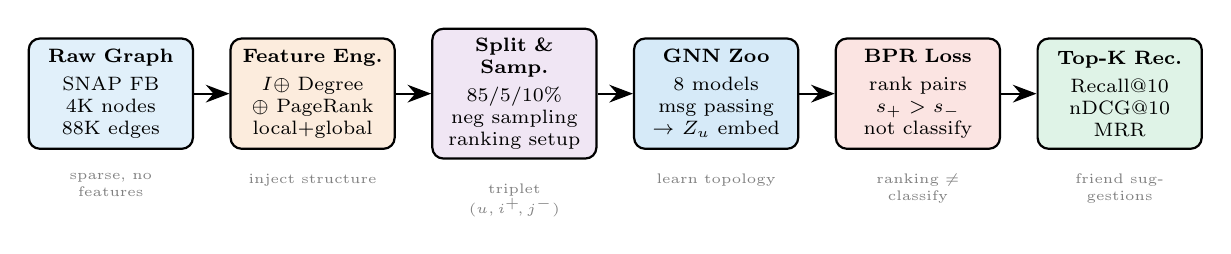
\begin{tikzpicture}[node distance=0.45cm]

\node[box style, fill=cblue!15, text width=1.85cm, minimum height=1.4cm] (s1) {
  \textbf{Raw Graph}\\[2pt]
  SNAP FB\\4K nodes\\88K edges};
\node[box style, fill=accent!15, text width=1.85cm, minimum height=1.4cm, right=of s1] (s2) {
  \textbf{Feature Eng.}\\[2pt]
  $I \oplus$ Degree\\$\oplus$ PageRank\\local+global};
\node[box style, fill=cpurple!15, text width=1.85cm, minimum height=1.4cm, right=of s2] (s3) {
  \textbf{Split \& Samp.}\\[2pt]
  85/5/10\%\\neg sampling\\ranking setup};
\node[box style, fill=cblue!20, text width=1.85cm, minimum height=1.4cm, right=of s3] (s4) {
  \textbf{GNN Zoo}\\[2pt]
  8 models\\msg passing\\$\to Z_u$ embed};
\node[box style, fill=gapred!15, text width=1.85cm, minimum height=1.4cm, right=of s4] (s5) {
  \textbf{BPR Loss}\\[2pt]
  rank pairs\\$s_+\!>\!s_-$\\not classify};
\node[box style, fill=fixgreen!15, text width=1.85cm, minimum height=1.4cm, right=of s5] (s6) {
  \textbf{Top-K Rec.}\\[2pt]
  Recall@10\\nDCG@10\\MRR};

\draw[arr style] (s1)--(s2);
\draw[arr style] (s2)--(s3);
\draw[arr style] (s3)--(s4);
\draw[arr style] (s4)--(s5);
\draw[arr style] (s5)--(s6);

\node[below=0.18cm of s1, font=\tiny, text width=1.85cm, align=center, text=gray]
  {sparse, no features};
\node[below=0.18cm of s2, font=\tiny, text width=1.85cm, align=center, text=gray]
  {inject structure};
\node[below=0.18cm of s3, font=\tiny, text width=1.85cm, align=center, text=gray]
  {triplet $(u,i^+\!,j^-)$};
\node[below=0.18cm of s4, font=\tiny, text width=1.85cm, align=center, text=gray]
  {learn topology};
\node[below=0.18cm of s5, font=\tiny, text width=1.85cm, align=center, text=gray]
  {ranking $\neq$ classify};
\node[below=0.18cm of s6, font=\tiny, text width=1.85cm, align=center, text=gray]
  {friend suggestions};

\end{tikzpicture}
\end{center}

\vspace{0.1em}

\begin{columns}[T]
\begin{column}{0.32\textwidth}
\begin{block}{\scriptsize\centering Structure as Feature}
\scriptsize No user profiles exist.
Degree (local) + PageRank (global) \textbf{inject topology} as learnable signals.
\end{block}
\end{column}
\begin{column}{0.32\textwidth}
\begin{block}{\scriptsize\centering Embeddings from Graphs}
\scriptsize GNNs propagate signals across hops.
Final $Z_u$ encodes \textbf{who a user is} inside the social graph.
\end{block}
\end{column}
\begin{column}{0.32\textwidth}
\begin{block}{\scriptsize\centering Rank, Don't Classify}
\scriptsize BPR forces $s_+ > s_-$ per triplet.
Output is a \textbf{ranked Top-K list}, not a binary link decision.
\end{block}
\end{column}
\end{columns}

\end{frame}



% ============ F11a: GCN FORWARD PASS ============
\begin{frame}
\frametitle{GCN Forward Pass \textbf{[O1]}}

\begin{block}{Step 1 --- Input: The Social Map}
\small
The graph $G$ is encoded as two matrices fed into the GCN:
\begin{itemize}
  \small
  \item \alert{\textbf{Feature Matrix}} $X \in \mathbb{R}^{n \times d}$: each row = one user's feature vector (Identity $\oplus$ Degree $\oplus$ PageRank).
  \item \alert{\textbf{Adjacency Matrix}} $A \in \mathbb{R}^{n \times n}$: encodes who is connected to whom.
\end{itemize}
\vspace{0.2em}
The initial node embedding is simply the feature matrix:
\begin{align*}
  H^{(0)} = X
\end{align*}
\end{block}

\vspace{0.2em}

\begin{exampleblock}{Step 2 --- Message Passing: Learn from Neighbours}
\small
At each layer $l$, every node \textbf{aggregates its neighbours' embeddings}, applies a learnable weight matrix $W^{(l)}$, and passes through a non-linearity:
\begin{align*}
  H^{(l+1)} = \sigma\!\left(\tilde{D}^{-1/2}\,\tilde{A}\,\tilde{D}^{-1/2}\,H^{(l)}\,W^{(l)}\right)
\end{align*}
\begin{itemize}
  \small
  \item $\tilde{A} = A + I$ \;--- self-loops added so each node includes itself.
  \item $\tilde{D}^{-1/2}\tilde{A}\tilde{D}^{-1/2}$ \;--- \alert{renormalisation} prevents high-degree nodes from dominating.
  \item \textbf{2 layers} $\Rightarrow$ each node sees its \alert{2-hop neighbourhood}.
  Final output: $Z = H^{(2)}$.
\end{itemize}
\end{exampleblock}

\end{frame}


% ============ F11b: DECODING & OPTIMIZATION ============
\begin{frame}
\frametitle{GCN Decoding and Optimization \textbf{[O1, O3]}}

\begin{exampleblock}{Step 3 --- Decoder: Score Every Candidate Link}
\small
After message passing, each node $u$ has a learned embedding $Z_u \in \mathbb{R}^{d}$ that encodes its \textbf{position and role} in the graph.\\[4pt]
A link score between any pair $(u, v)$ is computed via a simple \alert{dot product}:
\begin{align*}
  s_{uv} = Z_u^{\top} Z_v
\end{align*}
High score $\Rightarrow$ model believes a friendship is likely.
\textbf{No extra parameters needed.}
\end{exampleblock}

\vspace{0.25em}

\begin{alertblock}{Step 4 --- BPR Optimization: Learn to Rank}
\small
For each user $u$, sample a \alert{positive} friend $i^+$ and a \alert{negative} stranger $j^-$.
BPR forces $s_{ui} > s_{uj}$:
\begin{align*}
  \mathcal{L}_{\text{BPR}} = -\sum_{(u,\,i^+,\,j^-)} \ln\,\sigma\!\bigl(s_{ui} - s_{uj}\bigr)
\end{align*}
Gradients flow back through the decoder into $W^{(l)}$.
Adam updates weights adaptively:
\begin{align*}
  W^{(l)}_{\text{new}} = W^{(l)}_{\text{old}} - \eta\,\nabla_{W}\,\mathcal{L}_{\text{BPR}}
\end{align*}
Early stopping fires when Val AUC stagnates (patience = 25).
\end{alertblock}

\end{frame}


% ============ F11c: GCN INTUITION SUMMARY ============
\begin{frame}
\frametitle{GCN Intuition --- The Full Picture}

\begin{center}
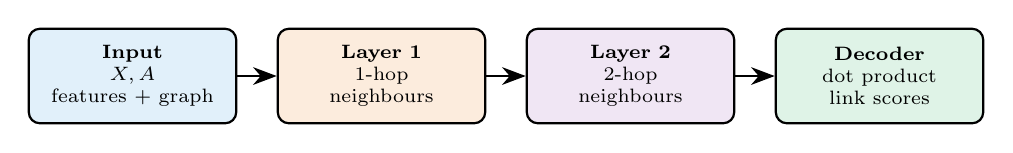
\begin{tikzpicture}[node distance=0.5cm]
\node[box style, fill=cblue!15,    text width=2.4cm, minimum height=1.2cm] (n1)
  {\textbf{Input}\\$X, A$\\features + graph};
\node[box style, fill=accent!15,   text width=2.4cm, minimum height=1.2cm, right=of n1] (n2)
  {\textbf{Layer 1}\\1-hop\\neighbours};
\node[box style, fill=cpurple!15,  text width=2.4cm, minimum height=1.2cm, right=of n2] (n3)
  {\textbf{Layer 2}\\2-hop\\neighbours};
\node[box style, fill=fixgreen!15, text width=2.4cm, minimum height=1.2cm, right=of n3] (n4)
  {\textbf{Decoder}\\dot product\\link scores};
\draw[arr style] (n1)--(n2);
\draw[arr style] (n2)--(n3);
\draw[arr style] (n3)--(n4);
\end{tikzpicture}
\end{center}

\vspace{0.3em}

\begin{columns}[T]
\begin{column}{0.48\textwidth}
\begin{block}{What GCN Learns}
\small
\begin{itemize}
  \item \alert{Layer 1:} Who are my direct friends?
  \item \alert{Layer 2:} Who are my friends' friends?
  \item \alert{$Z_u$:} A compressed fingerprint of node $u$'s \textbf{structural role} in the graph.
\end{itemize}
\end{block}
\end{column}
\begin{column}{0.48\textwidth}
\begin{alertblock}{Why This Works for Recommendation}
\small
\begin{itemize}
  \item Similar users end up with \alert{similar embeddings}.
  \item Dot product ranks true friends \textbf{higher} than strangers.
  \item BPR ensures the model learns \textbf{order}, not just existence.
\end{itemize}
\end{alertblock}
\end{column}
\end{columns}

\vspace{0.2em}

\begin{block}{}
\small\centering
\textit{``GCN turns a sparse graph into a dense, rankable embedding space --- structure becomes signal.''}
\end{block}

\end{frame}

% ============ F?: OTHER MODELS — MESSAGE PASSING ============
\begin{frame}
\frametitle{Model Zoo: Message Passing Variants \textbf{[O1]}}

\begin{block}{Starting Point: GCN}
\small
GCN averages neighbours uniformly.
Each model below addresses a \alert{specific limitation} of this design.
\end{block}

\vspace{0.25em}

\begin{columns}[T]

\begin{column}{0.48\textwidth}

\begin{exampleblock}{GraphConv (Vanilla GNN)}
\small
\textbf{Idea:} Separate self and neighbour signals.\\
\textbf{Change:} Different weights for node and neighbours.\\
\textbf{Why:} \alert{Preserves node identity}.\\
\textit{Think:} “Learn from neighbours, but stay distinct.”
\end{exampleblock}

\vspace{0.2em}

\begin{exampleblock}{GraphSAGE}
\small
\textbf{Idea:} Sample neighbours.\\
\textbf{Change:} Aggregate a subset, not all nodes.\\
\textbf{Why:} \alert{Scales to large graphs}.\\
\textit{Think:} “Ask a few neighbours, not everyone.”
\end{exampleblock}

\end{column}

\begin{column}{0.48\textwidth}

\begin{exampleblock}{GIN (Graph Isomorphism Network)}
\small
\textbf{Idea:} Use sum + MLP.\\
\textbf{Change:} Replace mean with learned function.\\
\textbf{Why:} \alert{Most expressive GNN}.\\
\textit{Think:} “Capture exact structure.”
\end{exampleblock}

\vspace{0.2em}

\begin{alertblock}{Key Takeaway}
\small
\begin{itemize}
\item GraphConv $\rightarrow$ better weighting  
\item GraphSAGE $\rightarrow$ scalability  
\item GIN $\rightarrow$ \alert{highest expressiveness}  
\end{itemize}
All improve over GCN for sparse graphs.
\end{alertblock}

\end{column}

\end{columns}

\end{frame}

% ============ F?: OTHER MODELS — ATTENTION & ADVANCED ============
\begin{frame}
\frametitle{Model Zoo: Attention and Lightweight Variants \textbf{[O1]}}

\begin{block}{Next Question: Which Neighbours Matter?}
\small
After aggregation, we ask: \alert{should all neighbours contribute equally?}
Attention models answer this.
LightGCN simplifies instead.
\end{block}

\vspace{0.25em}

\begin{columns}[T]

\begin{column}{0.48\textwidth}

\begin{exampleblock}{GAT}
\small
\textbf{Idea:} Learn neighbour importance.\\
\textbf{Change:} Attention weights instead of uniform averaging.\\
\textbf{Why:} Focus on \alert{important neighbours}.\\
\textit{Limit:} Static attention.
\end{exampleblock}

\vspace{0.2em}

\begin{exampleblock}{GATv2}
\small
\textbf{Idea:} Dynamic attention.\\
\textbf{Change:} Scores depend on node pairs.\\
\textbf{Why:} \alert{More flexible than GAT}.\\
\textit{Think:} “Context-aware attention.”
\end{exampleblock}

\end{column}

\begin{column}{0.48\textwidth}

\begin{exampleblock}{TransformerConv}
\small
\textbf{Idea:} Transformer-style attention.\\
\textbf{Change:} Query–key similarity.\\
\textbf{Why:} Captures \alert{complex relations}.\\
\textit{Think:} “Transformer on graphs.”
\end{exampleblock}

\vspace{0.2em}

\begin{alertblock}{LightGCN}
\small
\textbf{Idea:} Remove weights and activations.\\
\textbf{Change:} Only propagation remains.\\
\textbf{Why:} \alert{Fastest and lightweight}.\\
\textit{Tradeoff:} Weak structural learning.
\end{alertblock}

\end{column}

\end{columns}

\end{frame}

% ============ F12: BPR vs BCE ============
\begin{frame}
\frametitle{Methodology: BPR Loss vs BCE Loss \textbf{[O3]}}
\begin{columns}[T]
\begin{column}{0.48\textwidth}
\begin{alertblock}{BCE Loss (Classification)}
Treats each edge independently.\\
$\mathcal{L} = -[y\log\hat{y} + (1{-}y)\log(1{-}\hat{y})]$\\[4pt]
Problem: assigns 0.6 to both real friend AND stranger.
Recall@10 stays poor --- relative ordering never learned.
\end{alertblock}
\end{column}
\begin{column}{0.48\textwidth}
\begin{exampleblock}{BPR Loss (Ranking)}
Evaluates PAIRS: forces real friend score $>$ stranger.\\
$\mathcal{L} = -\log\sigma(\hat{y}_{ui} - \hat{y}_{uj})$\\[4pt]
Model explicitly learns to rank, not classify.
\end{exampleblock}
\end{column}
\end{columns}
\vspace{0.5em}
\alert{``Moving from BCE to BPR is not an implementation detail --- it is a fundamental paradigm shift from classification to personalised recommendation.''}\\[4pt]
\textbf{[O3 addressed --- ranking loss fully justified]}
\end{frame}

% ============ F22a: LEARNING DYNAMICS ============
\begin{frame}
\frametitle{Learning Dynamics --- Training vs Validation}

\begin{columns}[T]

\begin{column}{0.60\textwidth}
\begin{center}

\includegraphics[width=\textwidth, height=0.30\textheight, keepaspectratio]{learning_curves_gnn.png}\\
{\tiny \textbf{GNN} --- BPR Loss and Val AUC/AP vs Epochs}
\end{center}
\vspace{0.1em}
\begin{center}

\includegraphics[width=\textwidth, height=0.30\textheight, keepaspectratio]{learning_curves_gcn.png}\\
{\tiny \textbf{GCN} --- stable convergence, Val AUC $\approx$ 0.93}
\end{center}
\end{column}

\begin{column}{0.38\textwidth}

\begin{block}{What We Observe}
\small
\begin{itemize}
  \item Train loss \alert{decreases steadily} across all models.
  \item Val loss drops then \alert{stabilises} --- no divergence.
  \item Small train--val gap $\Rightarrow$ \alert{good generalisation}.
  \item Val AUC and AP \textbf{converge smoothly} from epoch 1.
\end{itemize}
\end{block}

\vspace{0.2em}

\begin{exampleblock}{Key Insight}
\small
\begin{itemize}
  \item Meaningful patterns learned \textbf{within first 20 epochs}.
  \item Later epochs show \alert{diminishing returns}.
  \item \textbf{GNN} converges fastest to highest Val AUC=0.933.
  \item \textbf{GAT} oscillates --- static attention struggles with sparse graphs.
\end{itemize}
\end{exampleblock}

\end{column}

\end{columns}

\end{frame}


% ============ F22b: REGULARIZATION & STABILITY ============
\begin{frame}
\frametitle{Preventing Overfitting --- Model Stability}

\begin{columns}[T]

\begin{column}{0.55\textwidth}
\begin{center}

\includegraphics[width=\textwidth, height=0.32\textheight, keepaspectratio]{learning_curves_gat.png}\\
{\tiny \textbf{GAT} --- oscillating loss, \alert{overfitting risk} visible after epoch 20}
\end{center}

\vspace{0.15em}

\begin{alertblock}{Final Takeaway}
\small
\begin{itemize}
  \item \textbf{GNN / GCN:} stable, well-regularised, reach \alert{optimal performance} before overfitting fires.
  \item \textbf{GAT:} train loss $\ll$ val loss after ep 20 --- \alert{early stopping critical}.
  \alert{Early stopping} saved 50--100 wasted epochs across all models.
\end{itemize}
\end{alertblock}
\end{column}

\begin{column}{0.42\textwidth}

\begin{block}{Regularisation Techniques Used}
\small
\begin{itemize}
  \item \alert{\textbf{Dropout = 0.3}} --- prevents node co-adaptation during message passing.
  \item \alert{\textbf{Adam Optimiser}} --- adaptive learning rate keeps updates stable.
  \item \alert{\textbf{Early Stopping}} --- patience = 25 on Val AUC;
  halts at best generalisation point.
\end{itemize}
\end{block}

\vspace{0.2em}

\begin{exampleblock}{Why It Matters}
\small
\begin{itemize}
  \item Controls \alert{overfitting} on a small 4K-node graph.
  \item Improves \alert{generalisation} to unseen test edges.
  \item Ensures \textbf{fair comparison} --- all 8 models stop at their own optimal epoch.
  \item GIN stops at ep 95; GATv2 runs to ep 175 --- patience reveals true capacity.
\end{itemize}
\end{exampleblock}

\end{column}

\end{columns}

\end{frame}

% ============ F13: CONTRIBUTIONS ============
\begin{frame}
\frametitle{Contributions \textbf{[O6]}}

\begin{columns}[T]

\begin{column}{0.32\textwidth}
\begin{block}{\centering $\Sigma$ Modular Pipeline}
\scriptsize\centering benchmark\_all.py: plug-and-play encoder swap, identical BPR + split + seed for all 8 models.
\end{block}
\vspace{0.2em}
\begin{block}{\centering API Deploy}
\scriptsize\centering fastapi\_inference.py: Top-K REST endpoint for real-time friend recommendation.
\end{block}
\vspace{0.2em}
\begin{exampleblock}{\centering Fair Benchmark}
\scriptsize\centering Identical seed=42, split, loss, and config across all 8 architectures --- first unified comparison.
\end{exampleblock}
\end{column}

\begin{column}{0.65\textwidth}
\begin{block}{XAI: Attention-Based Explainability \textbf{[O6]}}
\small
GATv2 assigns \alert{learnable attention weights} to every edge during message passing.
This lets us answer:
\begin{itemize}
  \small
  \item \textit{``Which neighbours influenced this recommendation?''}
  \item \textit{``Why was user X suggested to user Y?''}
\end{itemize}
\vspace{0.1em}
A \alert{2-hop attention subgraph} is extracted per prediction --- showing the exact structural evidence the model used.
\end{block}

\vspace{0.15em}

\begin{center}
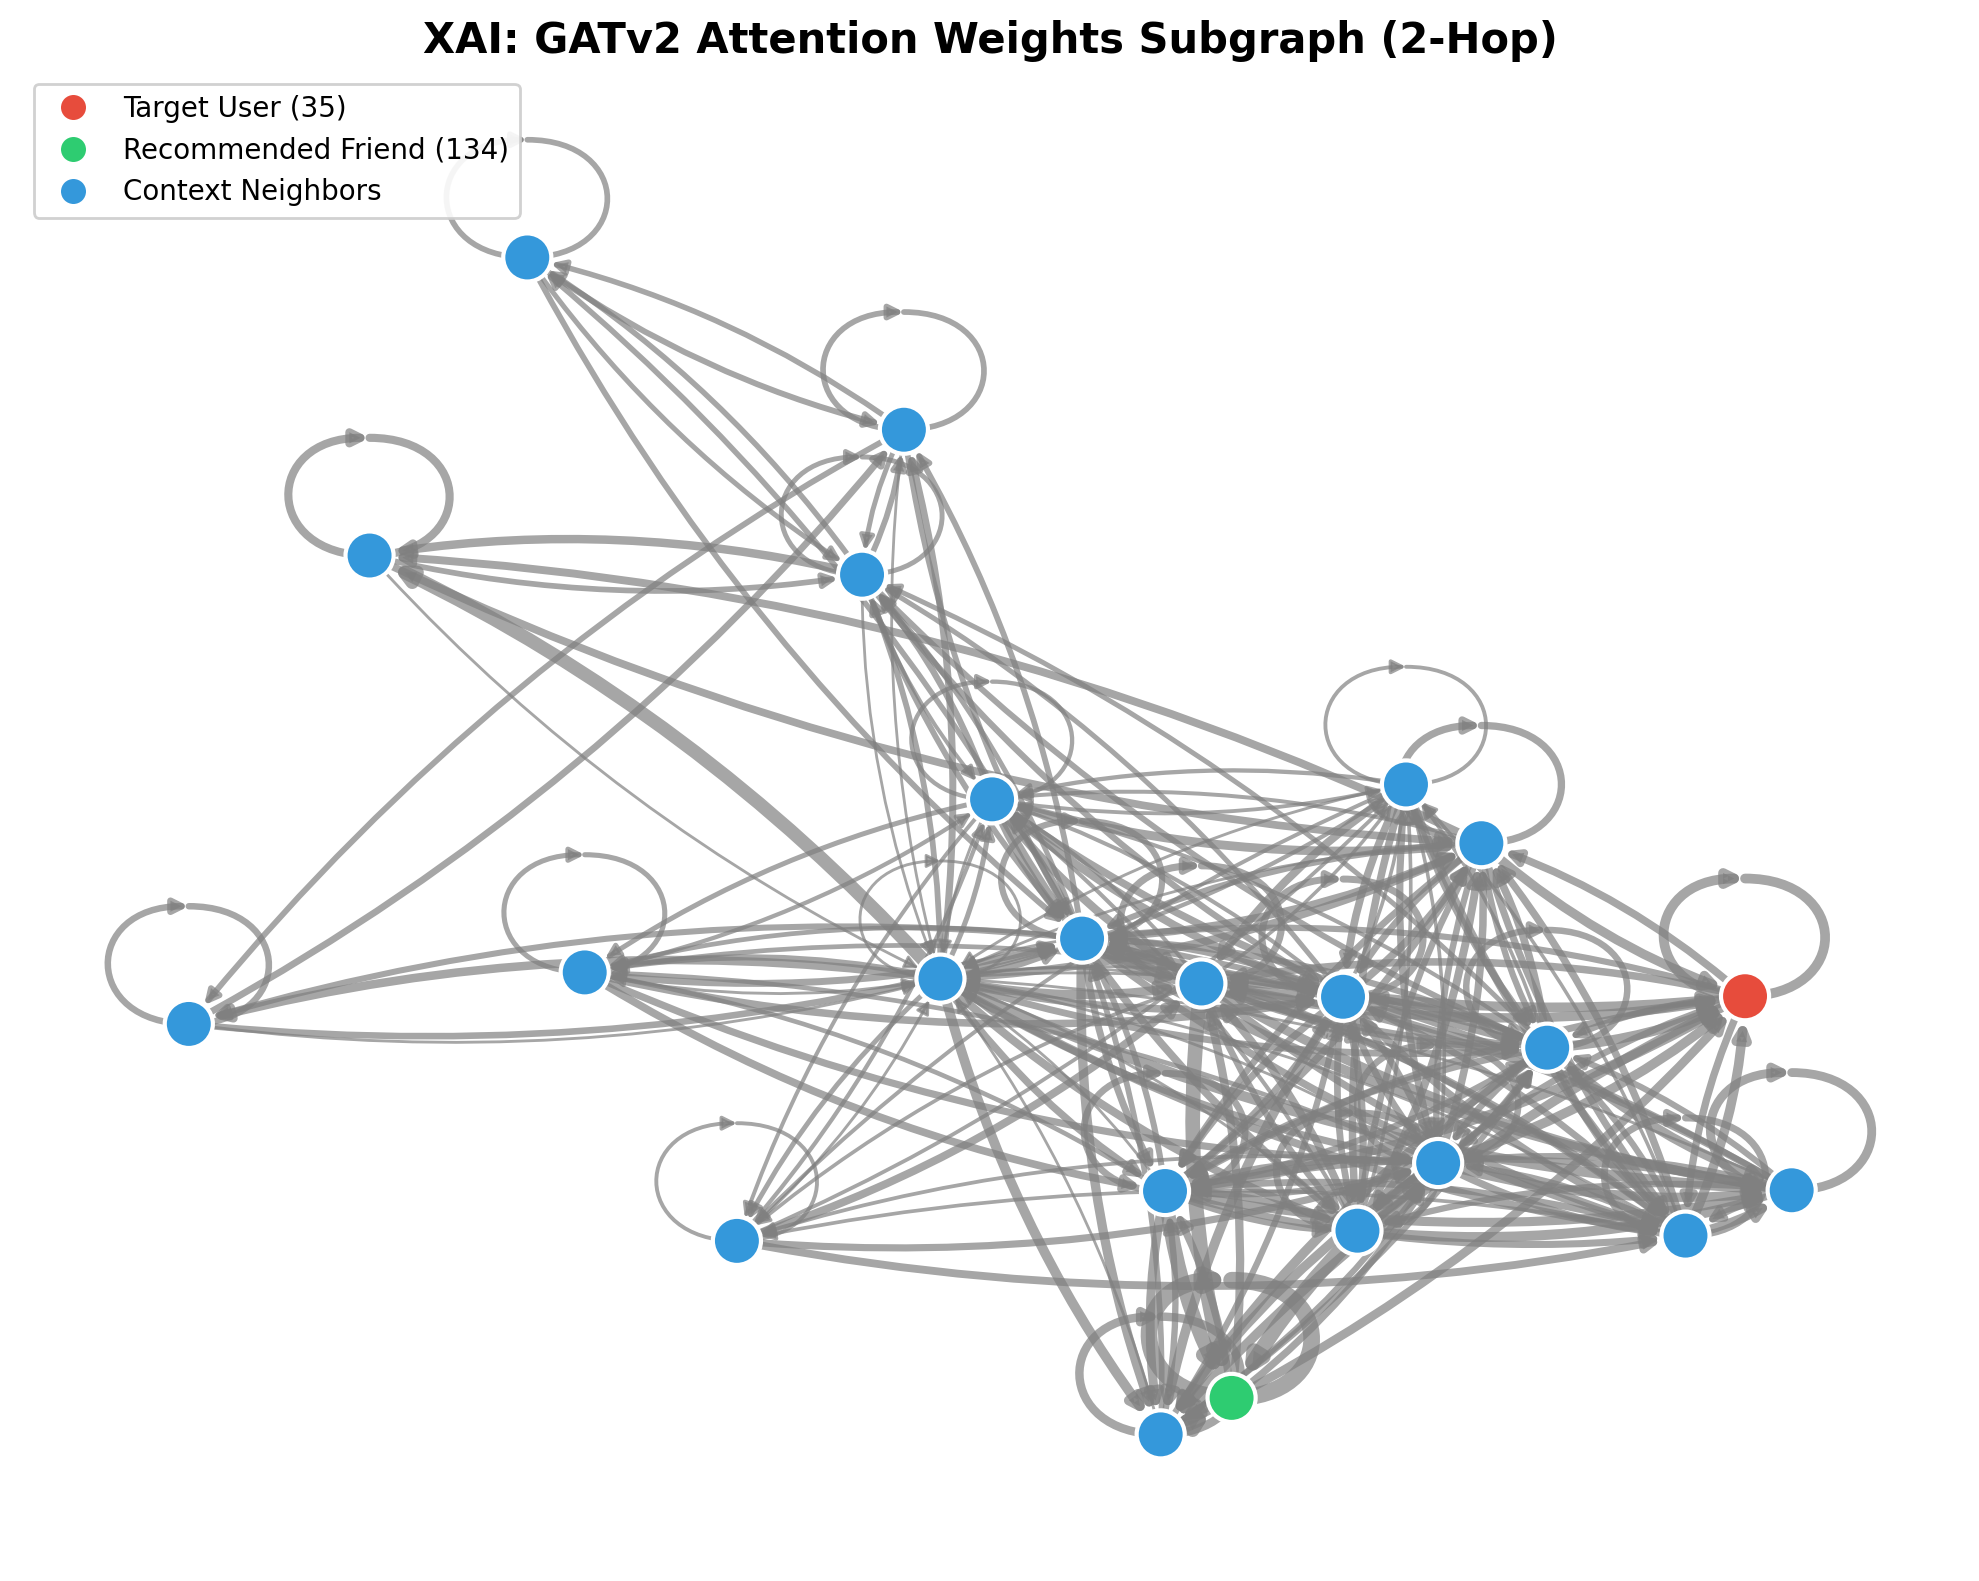
\includegraphics[width=\textwidth, height=0.38\textheight, keepaspectratio]{attention_subgraph.png}\\
{\tiny GATv2 XAI --- 2-hop attention subgraph for a sample recommendation \textbf{[O6]}}
\end{center}

\vspace{0.1em}

\begin{alertblock}{Key Insight}
\scriptsize
GNN recommendations are \alert{no longer a black box} --- attention weights expose the reasoning path, building trust in the system for real-world deployment.
\end{alertblock}

\end{column}

\end{columns}

\end{frame}

% ============ F14: t-SNE DASHBOARD ============
\begin{frame}
\frametitle{Qualitative Analysis: t-SNE Embedding Dashboard \textbf{[O5]}}
\begin{center}
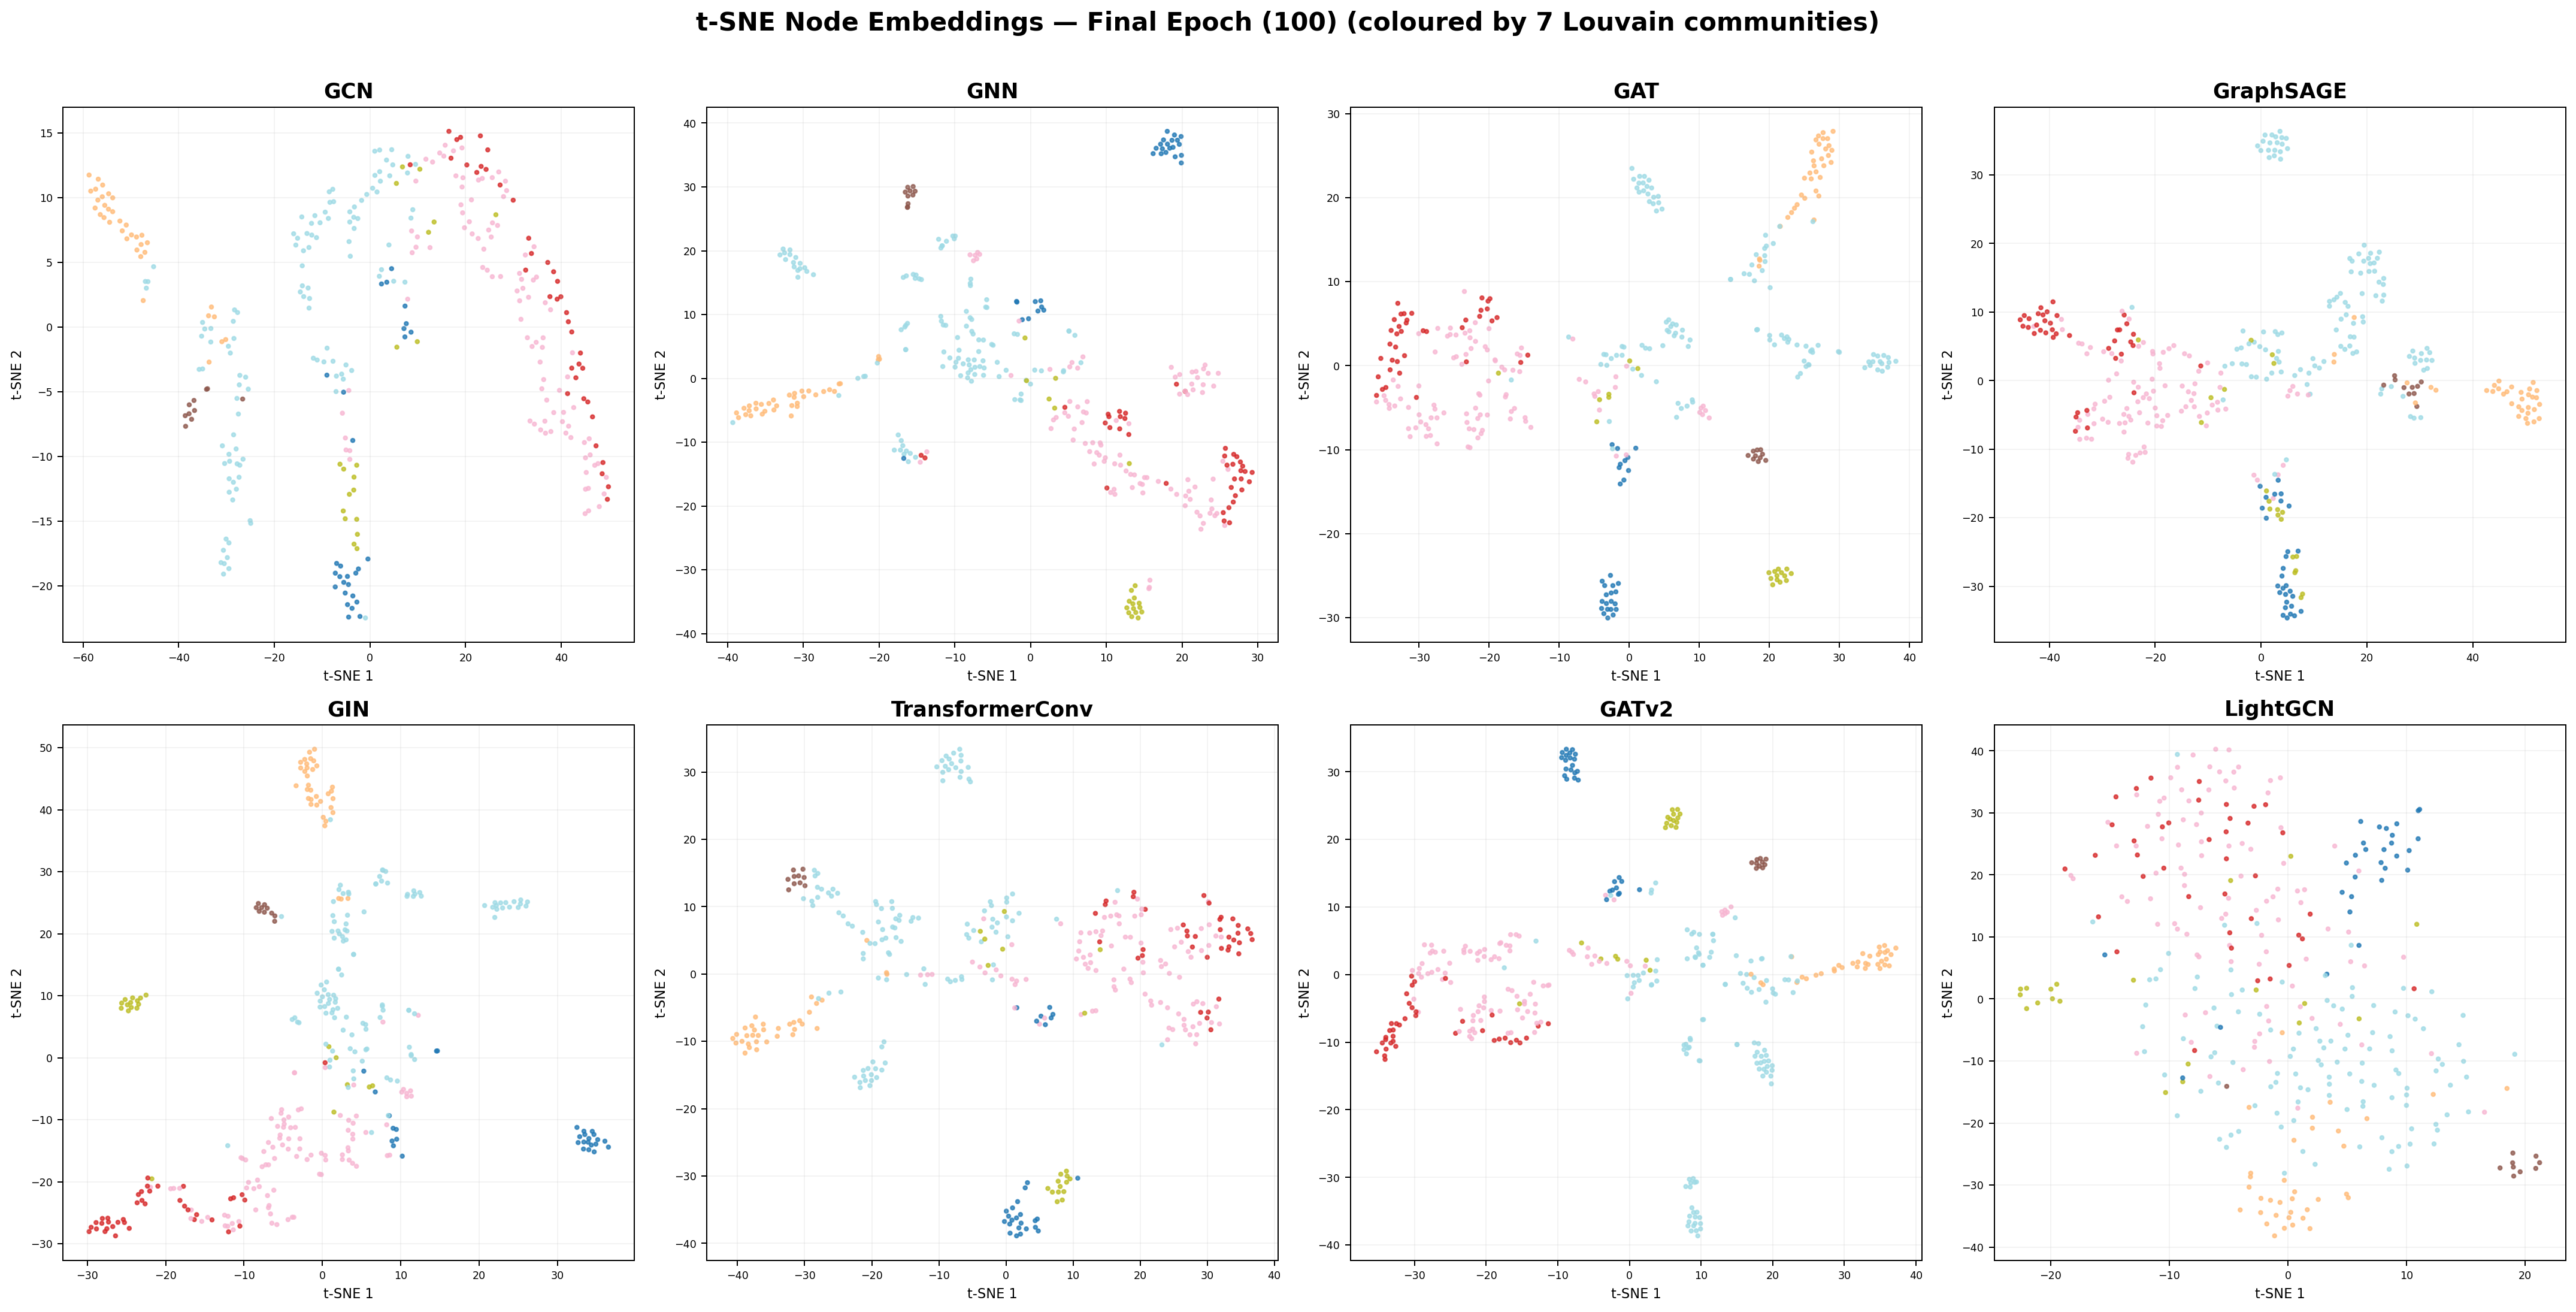
\includegraphics[width=\textwidth, height=0.75\textheight, keepaspectratio]{tsne_dashboard.png}
\end{center}
{\small t-SNE of final-epoch embeddings for all 8 models (7 Louvain communities).}
\begin{columns}[T]
\begin{column}{0.48\textwidth}
\begin{block}{Good Separation}
GNN, GIN, GATv2 --- tight clusters.
\end{block}
\end{column}
\begin{column}{0.48\textwidth}
\begin{alertblock}{\alert{LightGCN = complete blob.}}
Visually explains nDCG=0.221 despite AUC=0.875. Linear propagation cannot capture community topology.
\end{alertblock}
\end{column}
\end{columns}
\textbf{[O5 addressed]}
\end{frame}

% ============ F15: BEST vs WORST EMBEDDING ============
\begin{frame}
\frametitle{Embedding Quality vs Ranking Quality \textbf{[O5]}}
\begin{columns}[T]
\begin{column}{0.48\textwidth}
\centering
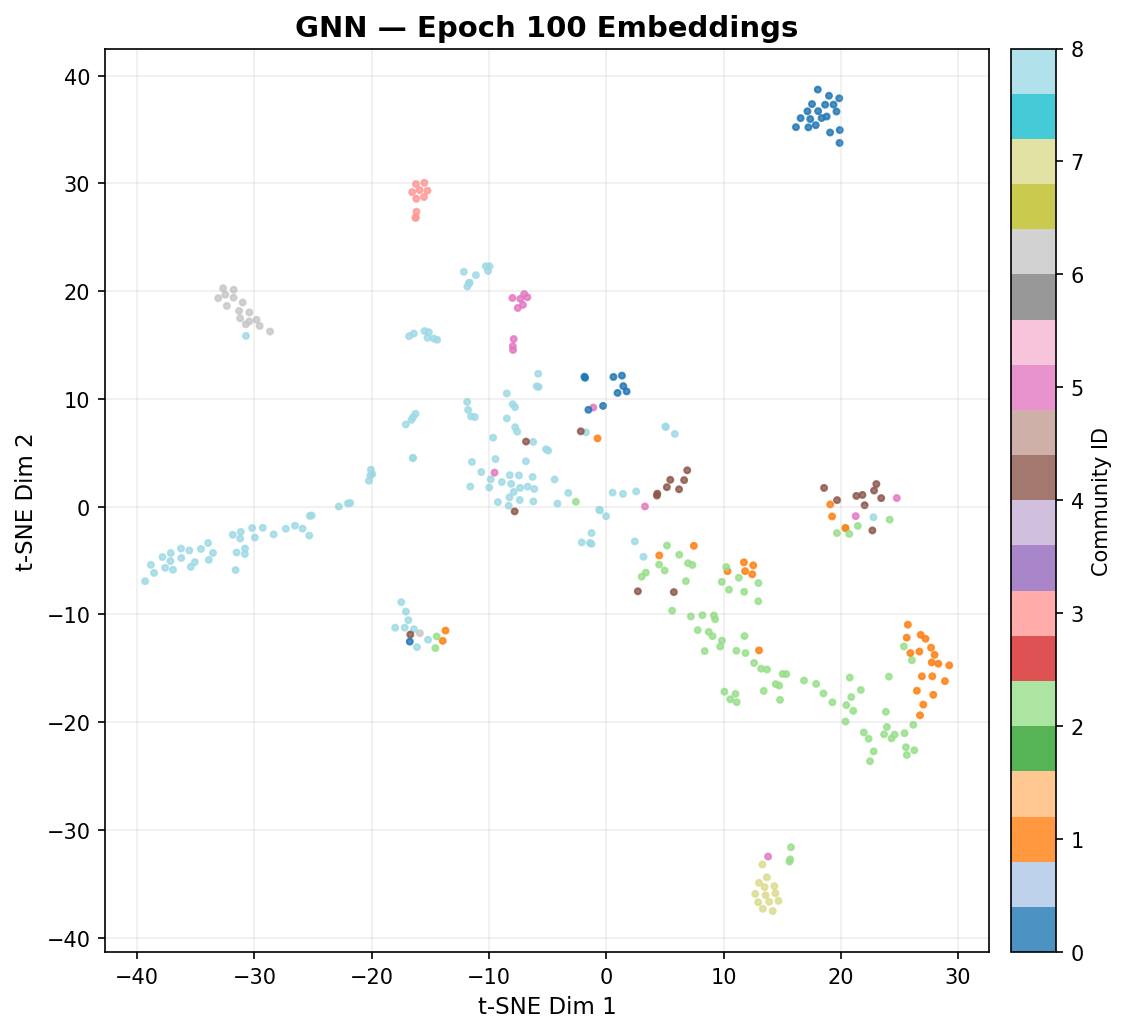
\includegraphics[width=\textwidth, height=0.4\textheight, keepaspectratio]{tsne_gnn.png}\\
\textbf{GNN} --- nDCG@10: \alert{0.422}\\
{\small Tight, well-separated community islands.}
\end{column}
\begin{column}{0.48\textwidth}
\centering
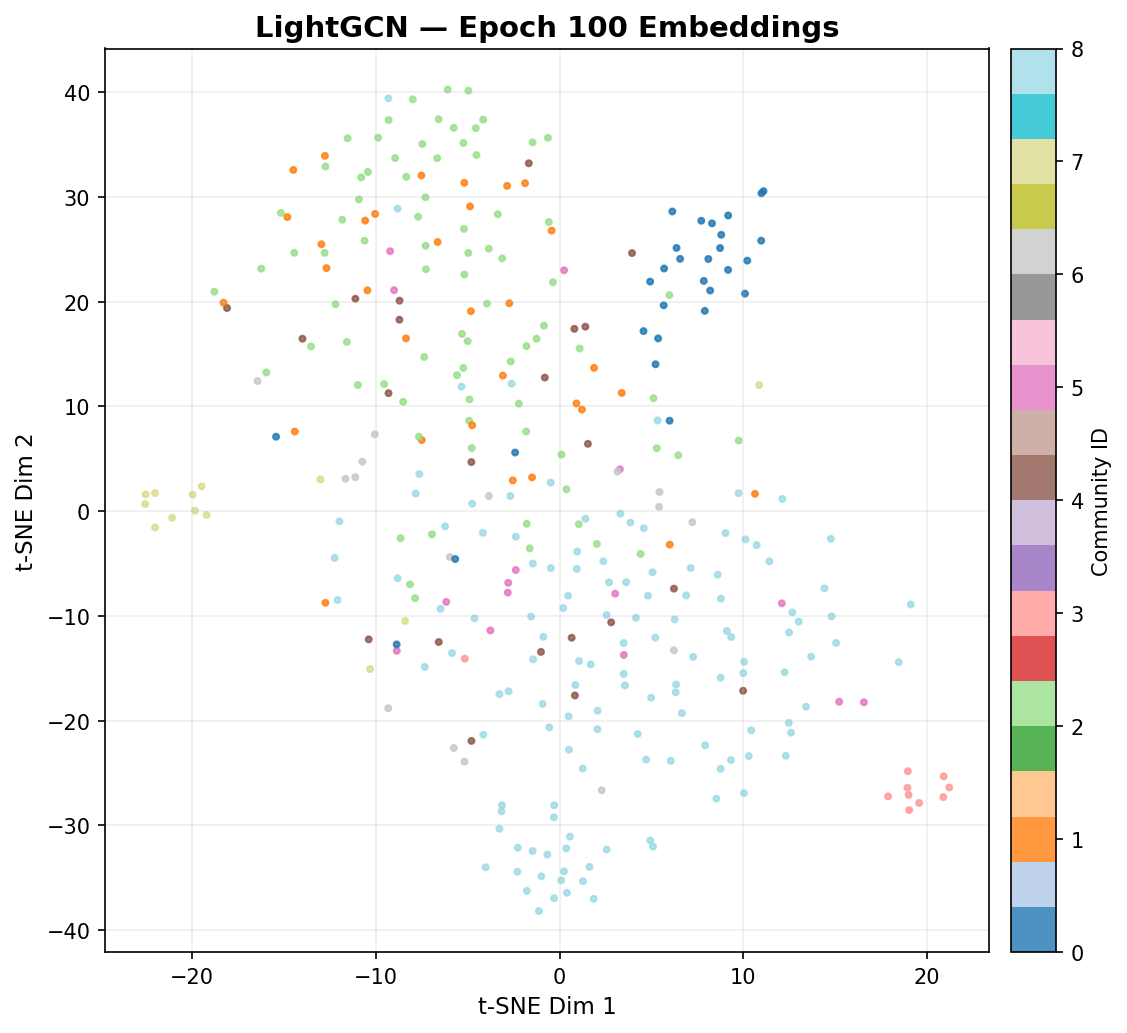
\includegraphics[width=\textwidth, height=0.4\textheight, keepaspectratio]{tsne_lightgcn.png}\\
\textbf{LightGCN} --- nDCG@10: \alert{0.221}\\
{\small Collapsed blob --- AUC=0.875 is misleading.}
\end{column}
\end{columns}
\vspace{0.3em}
\begin{alertblock}{Key Insight}
AUC measures \emph{if} a link exists.
nDCG measures if the model understands \emph{why} it exists. LightGCN's linear layers cannot capture community topology --- the t-SNE makes this failure visible to the human eye.
\end{alertblock}
\end{frame}

% ============ F16: GLOBAL BENCHMARK ============
\begin{frame}
\frametitle{Results: Global Benchmark \textbf{[O1]}}
\begin{center}
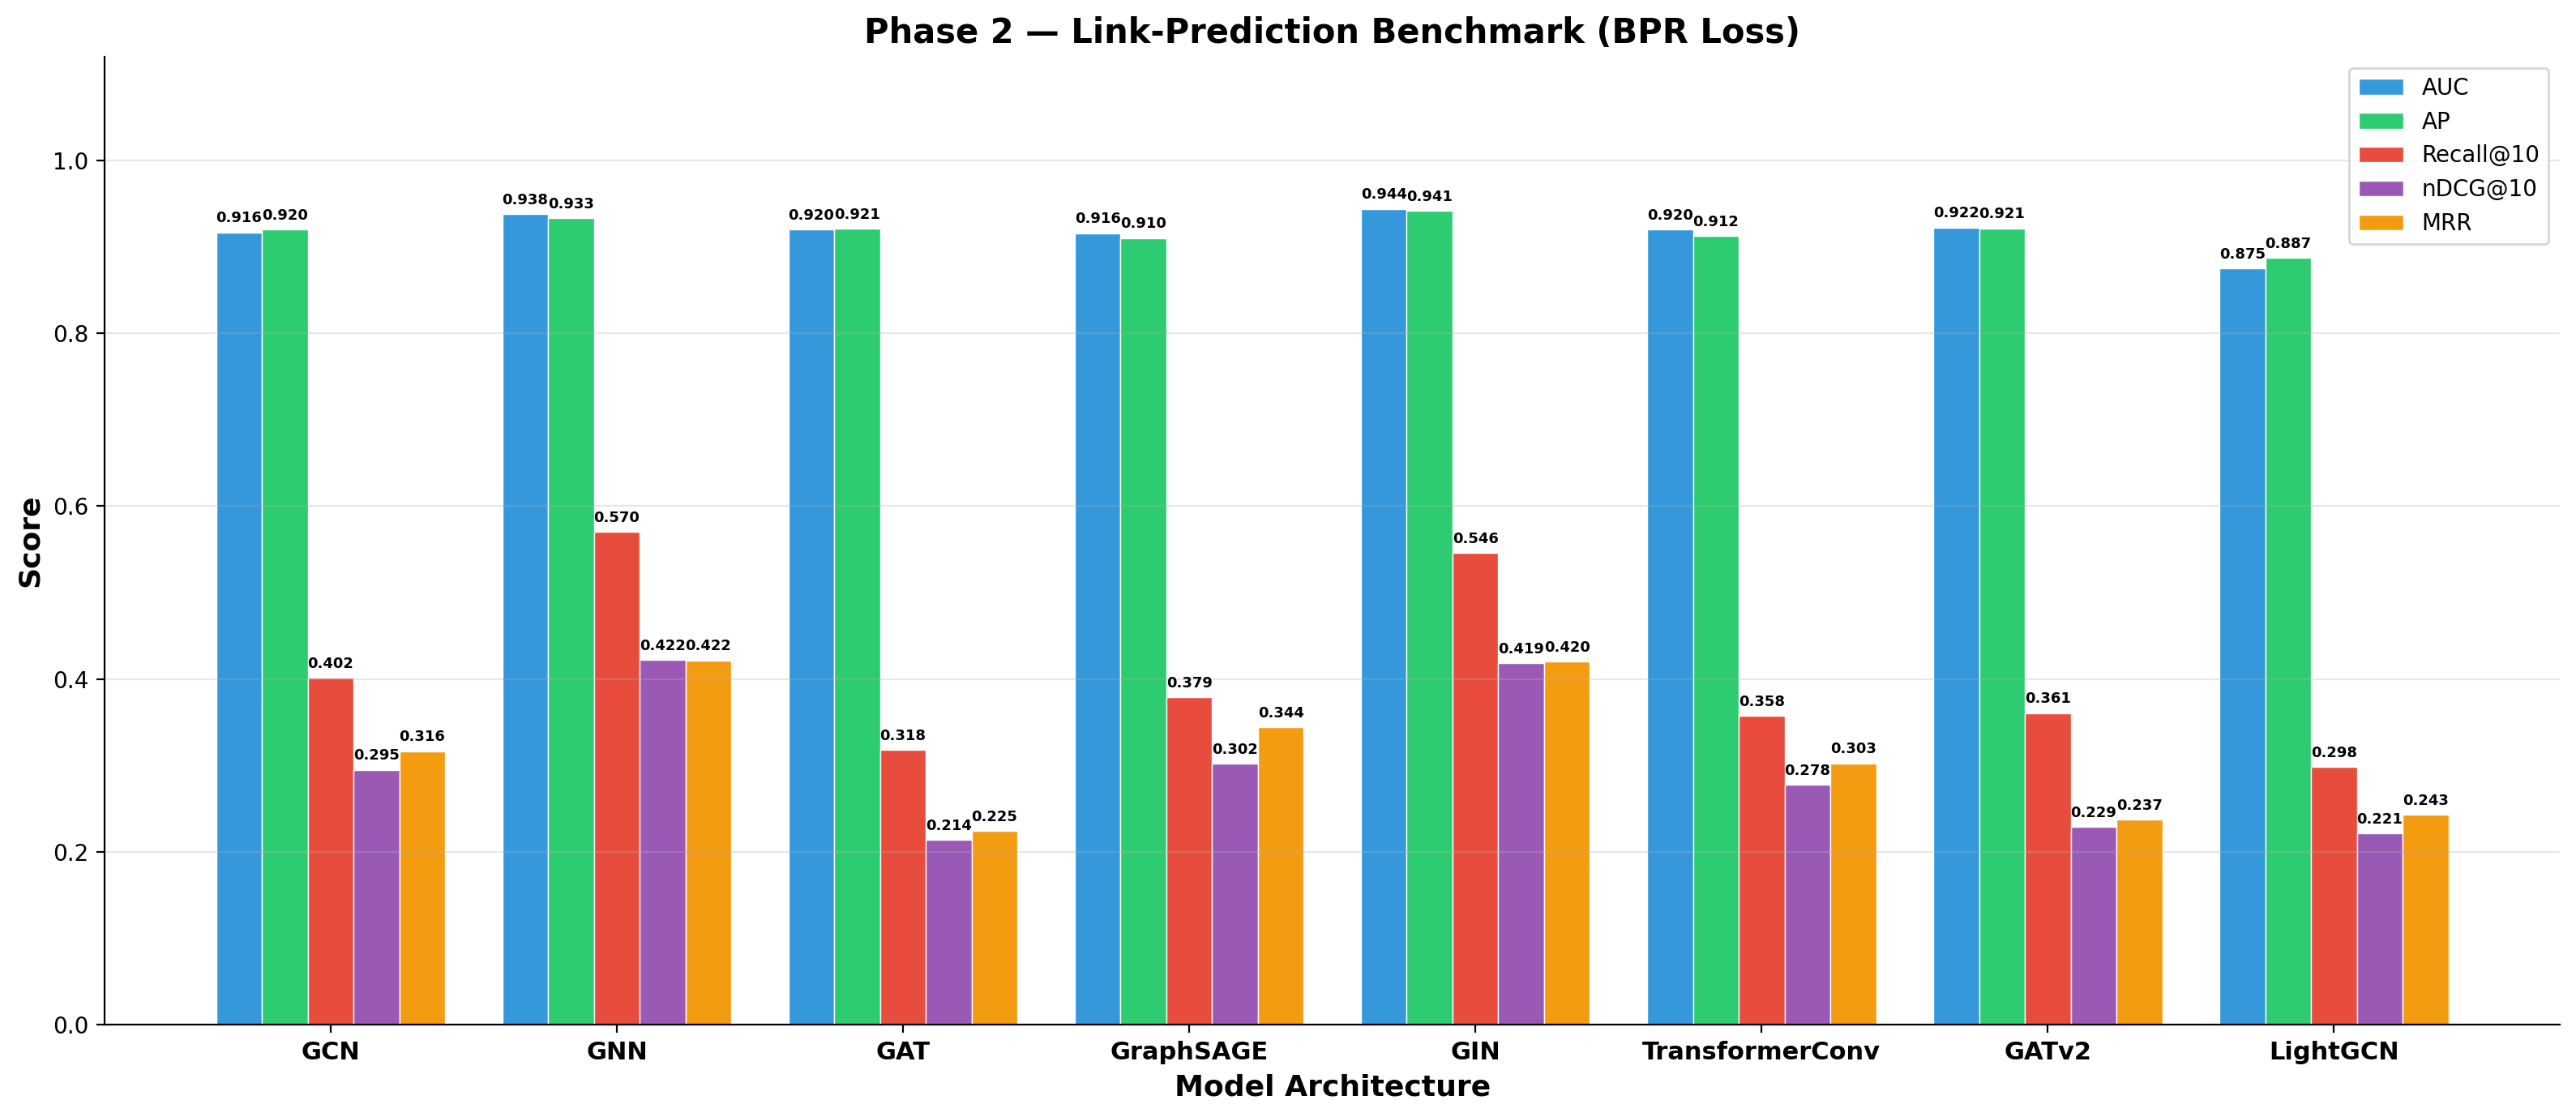
\includegraphics[width=\textwidth, height=0.72\textheight, keepaspectratio]{model_comparison.png}
\end{center}
\begin{columns}[T]
\begin{column}{0.32\textwidth}
\begin{block}{Winner}
\scriptsize GNN nDCG=0.422, GIN nDCG=0.419. MLP aggregation dominates.
\end{block}
\end{column}
\begin{column}{0.32\textwidth}
\begin{block}{Worst}
\scriptsize GAT nDCG=0.214. Static attention fails sparse neighbourhoods.
\end{block}
\end{column}
\begin{column}{0.32\textwidth}
\begin{block}{Misleading}
\scriptsize LightGCN AUC=0.875 but Recall@10=0.298. AUC is a poor proxy.
\end{block}
\end{column}
\end{columns}
\textbf{[O1 fully addressed]}
\end{frame}

% ============ F17: FULL BENCHMARK TABLE ============
\begin{frame}
\frametitle{Results: Full Benchmark Table \textbf{[O1,O3]}}
\renewcommand{\arraystretch}{1.3}
\scriptsize
\begin{center}
\begin{tabular}{lccccccc}
\toprule
\textbf{Model} & \textbf{AUC} & \textbf{AP} & \textbf{Recall@10} & \textbf{nDCG@10} & \textbf{MRR} & \textbf{Ep} & \textbf{ms/ep}\\
\midrule
GCN       & 0.916 & 0.920 & 0.402 & 0.295 & 0.316 & 171 &  7.3\\
\textbf{GNN} & \textbf{0.938} & \textbf{0.933} & \textbf{0.570} & \textbf{0.422} & \textbf{0.422} & \textbf{132} & \textbf{8.3}\\
\textcolor{gapred}{GAT} & \textcolor{gapred}{0.920} & \textcolor{gapred}{0.921} & \textcolor{gapred}{0.318} & \textcolor{gapred}{0.214} & \textcolor{gapred}{0.225} & \textcolor{gapred}{149} & \textcolor{gapred}{17.6}\\
GraphSAGE & 0.916 & 0.910 & 0.379 & 0.302 & 0.344 & 158 &  7.6\\
GIN       & 0.944 & 0.941 & 0.546 & 0.419 & 0.420 &  95 &  8.5\\
TConv     & 0.920 & 0.912 & 0.358 & 0.278 & 0.303 &  91 & 12.4\\
GATv2     & 0.922 & 0.921 & 0.361 & 0.229 & 0.237 & 175 & 29.0\\
LightGCN  & 0.875 & 0.887 & 0.298 & 0.221 & 0.243 &  32 &  5.3\\
\bottomrule
\end{tabular}
\end{center}
\footnotesize All runs: BPR loss, seed=42, patience=25, Adam, hidden=64.
\end{frame}

% ============ F18: ACCURACY vs EFFICIENCY ============
\begin{frame}
\frametitle{Results: Accuracy vs Efficiency \textbf{[O4]}}
\begin{center}
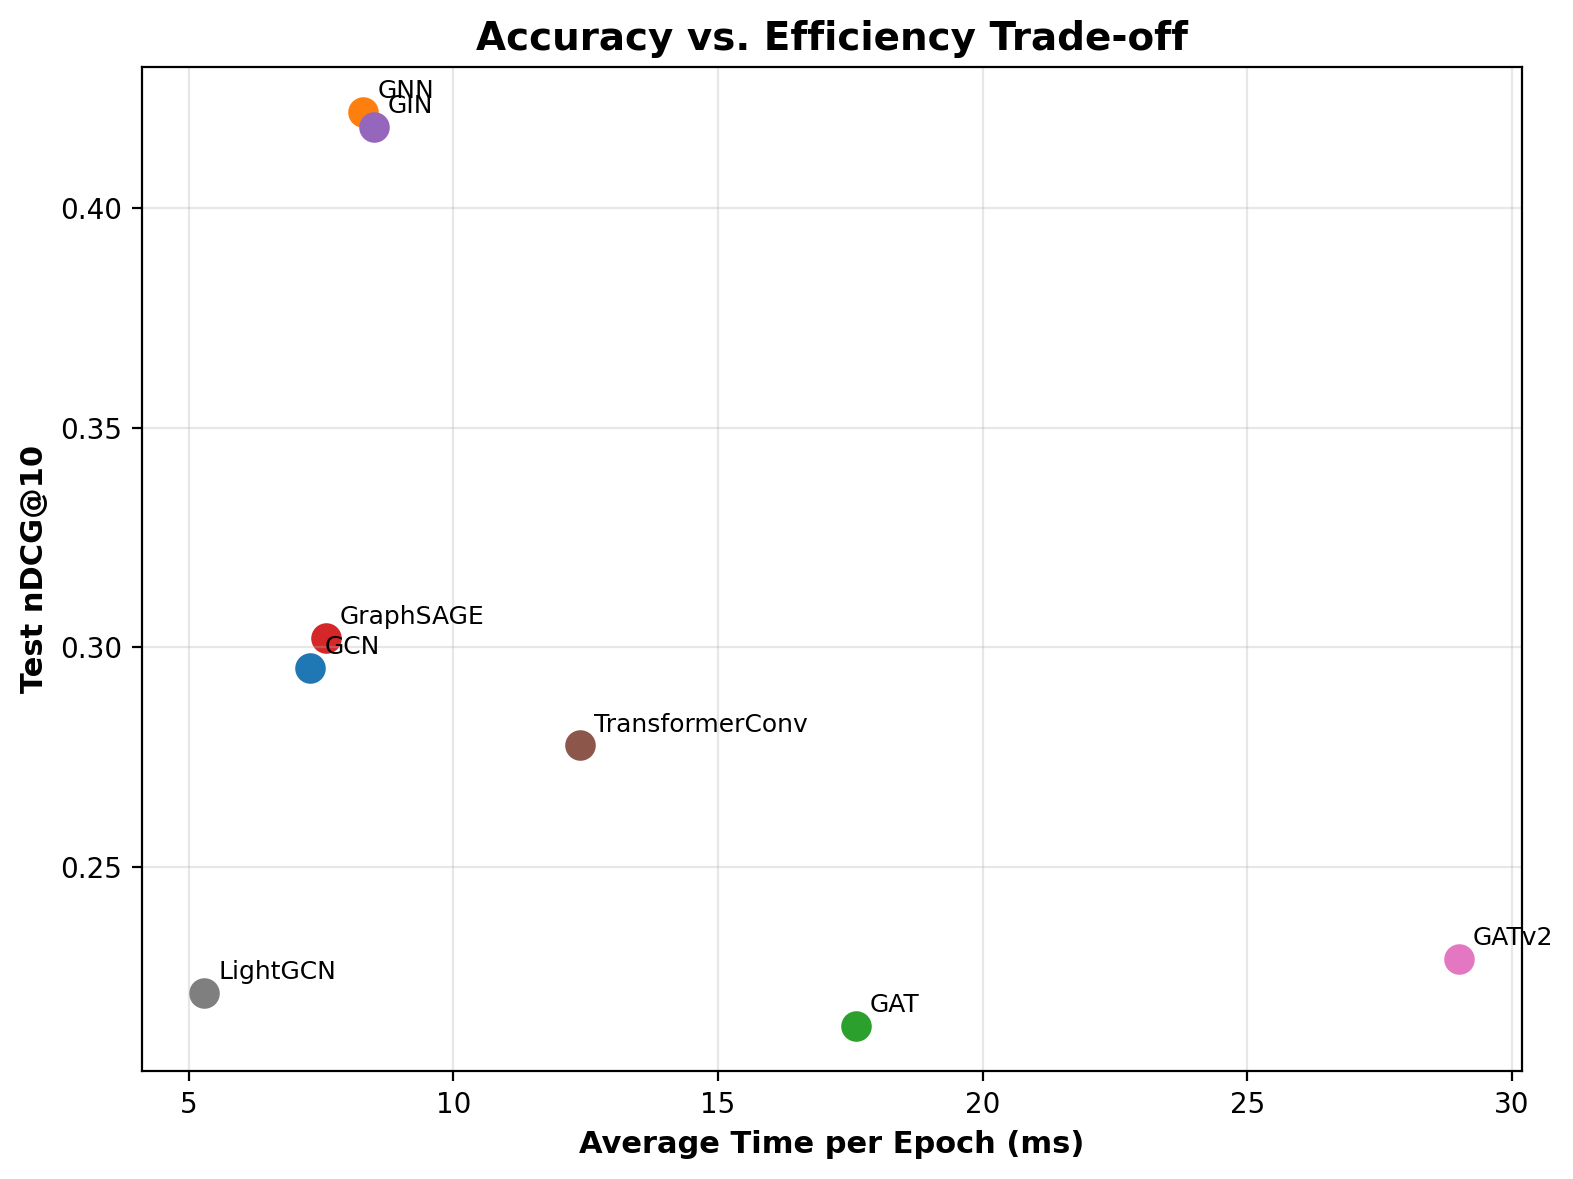
\includegraphics[width=0.9\textwidth, height=0.72\textheight, keepaspectratio]{efficiency_tradeoff.png}
\end{center}
\begin{itemize}
\item \textbf{Pareto Front}: GNN (8.3ms, 0.422) and GIN (8.5ms, 0.419) --- maximum accuracy at minimum cost. Production sweet spot.
\item \textbf{Scale Choice}: LightGCN (5.3ms, 22K params) --- fastest, minimal memory. Use when latency $>$ accuracy.
\item \textbf{Poor ROI}: GATv2 (29ms, 425K params, nDCG=0.229) --- 3.5$\times$ slower than GNN for half the ranking quality.
\end{itemize}
\textbf{[O4 addressed --- Pareto frontier mapped]}
\end{frame}

% ============ F19: COLD-START ============
\begin{frame}
\frametitle{Results: Cold-Start Analysis --- New vs Established Users \textbf{[O1]}}
\begin{center}
\IfFileExists{cold_start_chart.png}{%
  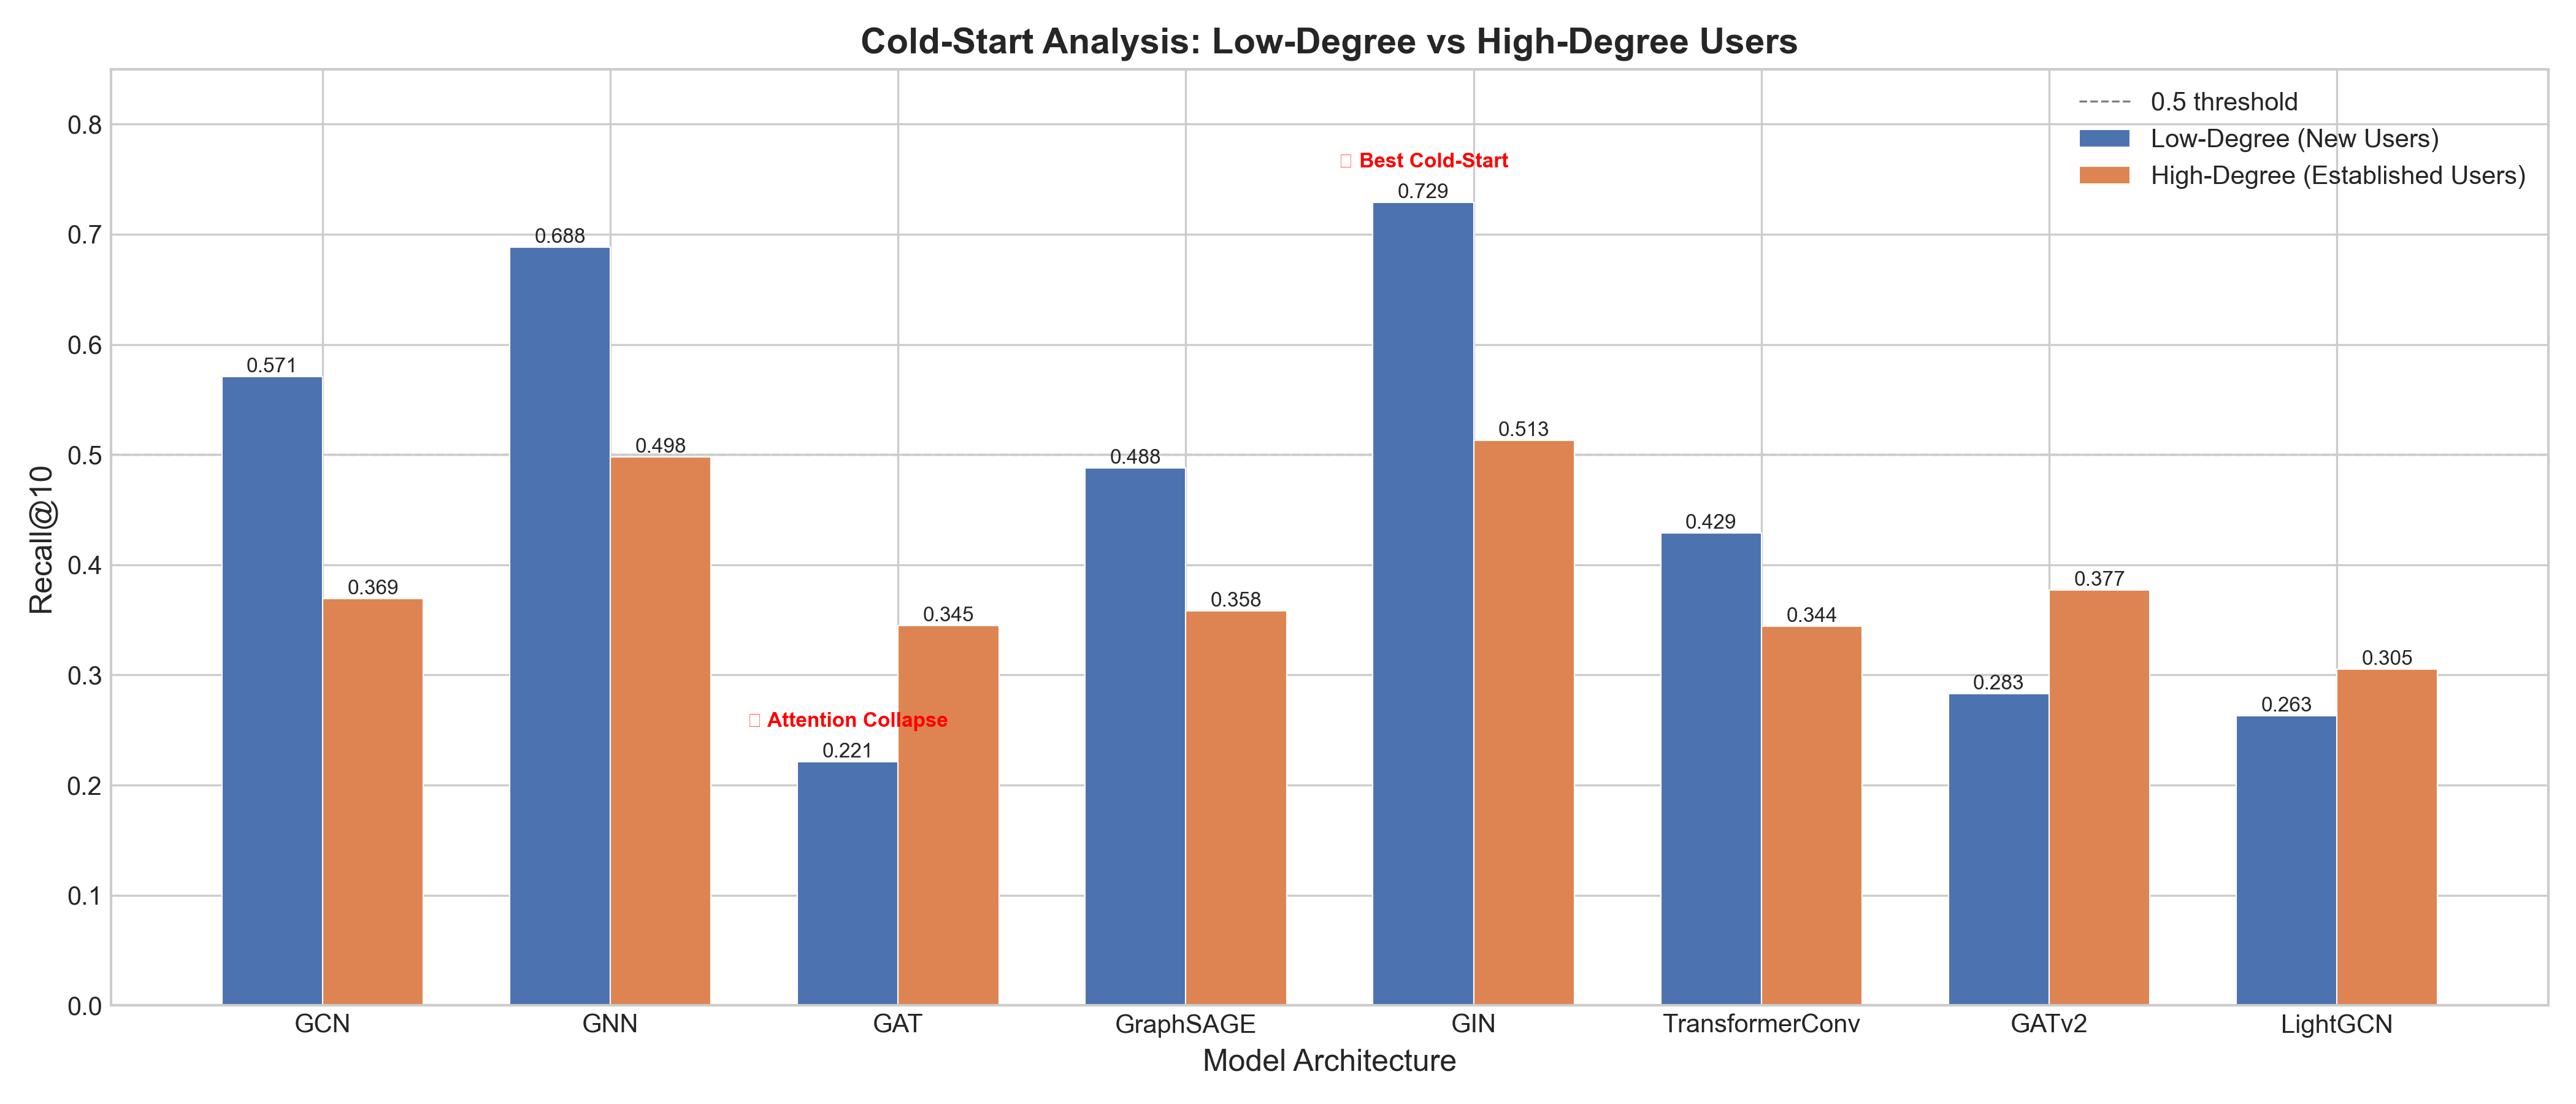
\includegraphics[width=\textwidth, height=0.50\textheight, keepaspectratio]{cold_start_chart.png}%
}{%
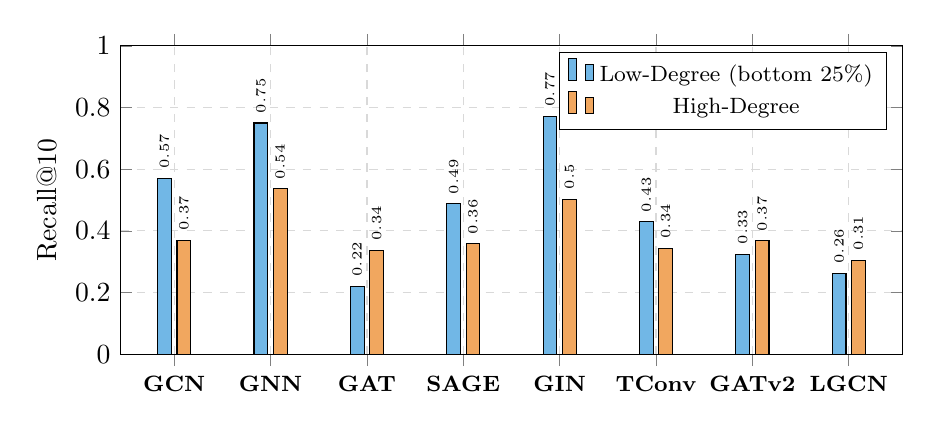
\begin{tikzpicture}
\begin{axis}[ybar, width=0.95\textwidth, height=5.5cm,
  bar width=5pt, ylabel={Recall@10},
  symbolic x coords={GCN,GNN,GAT,SAGE,GIN,TConv,GATv2,LGCN},
  xtick=data,
  xticklabel style={font=\footnotesize\bfseries},
  ymin=0, ymax=1.0,
  legend style={at={(0.98,0.98)},anchor=north east,font=\footnotesize},
  grid=major, grid style={dashed,gray!30},
  nodes near coords,
  every node near coord/.append style={font=\tiny,rotate=90,anchor=west},
  enlarge x limits=0.08]
\addplot[fill=cblue!70] coordinates {
  (GCN,0.5708)(GNN,0.7500)(GAT,0.2208)(SAGE,0.4875)
  (GIN,0.7708)(TConv,0.4292)(GATv2,0.3250)(LGCN,0.2625)};
\addplot[fill=accent!70] coordinates {
  (GCN,0.3694)(GNN,0.5361)(GAT,0.3368)(SAGE,0.3579)
  (GIN,0.5030)(TConv,0.3439)(GATv2,0.3676)(LGCN,0.3052)};
\legend{Low-Degree (bottom 25\%),High-Degree}
\end{axis}
\end{tikzpicture}%
}
\end{center}
\begin{columns}[T]
\begin{column}{0.48\textwidth}
\begin{block}{Key Finding}
\scriptsize GIN Low-Deg=0.771 (best). GNN Low-Deg=0.750 (second).
MLP aggregation handles sparsity without neighbour-count dependence.
\end{block}
\end{column}
\begin{column}{0.48\textwidth}
\begin{alertblock}{Attention Collapse}
\scriptsize GAT Low-Deg=0.221. GATv2 Low-Deg=0.325. Attention weights require multiple neighbours.
For users with 1--2 connections: attention = random noise.
\end{alertblock}
\end{column}
\end{columns}
{\small\alert{Surprising: Low-Degree Recall $>$ High-Degree for most models.
Popular users are HARDER to rank --- concentration-of-competition effect: Top-10 selected from a far larger candidate pool.}}
\end{frame}

% ============ F20: ABLATION — FEATURE HYDRATION ============
\begin{frame}
\frametitle{Ablation Study: Does Feature Engineering Matter? \textbf{[O2]}}
\begin{columns}[T]
\begin{column}{0.52\textwidth}
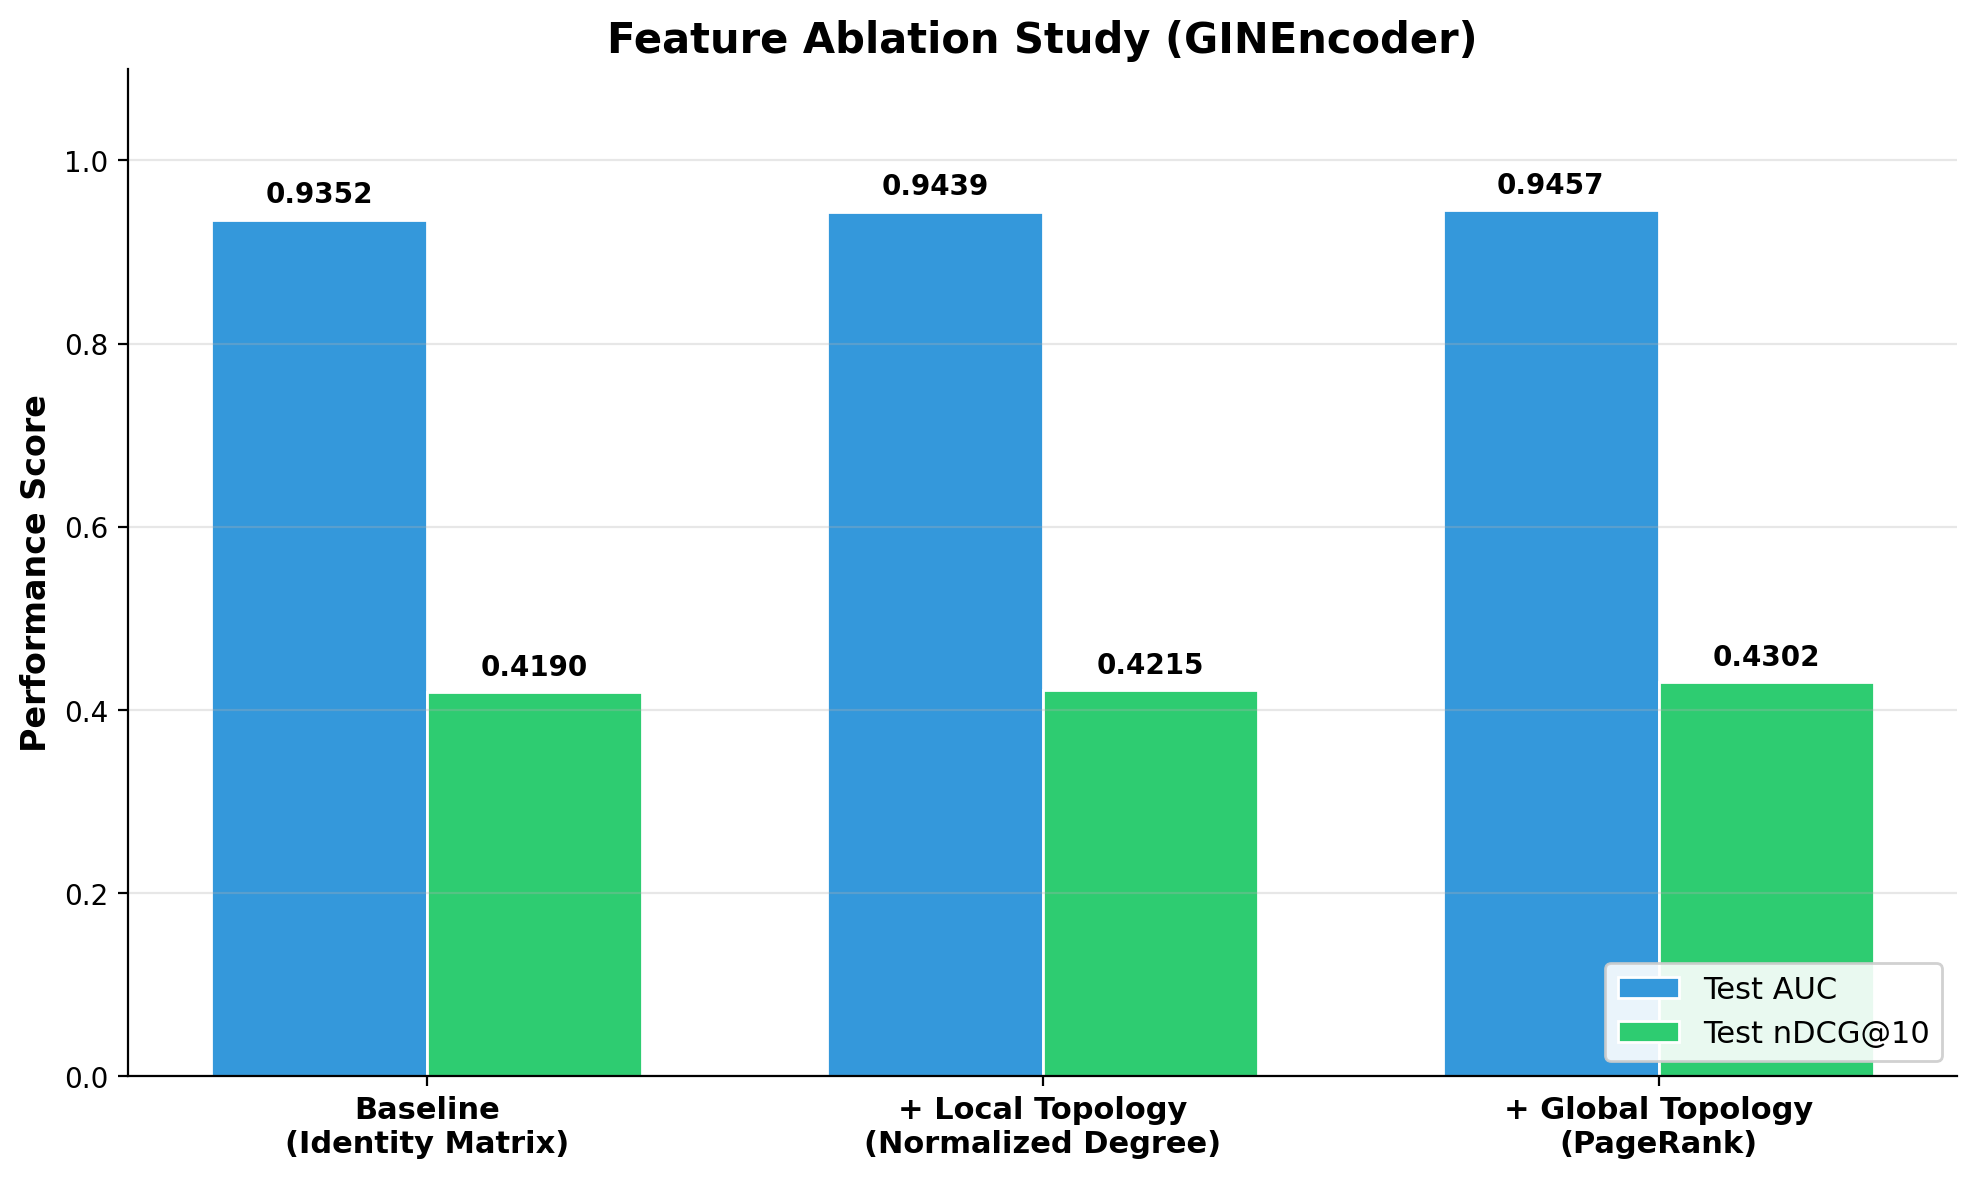
\includegraphics[width=\textwidth, height=0.42\textheight, keepaspectratio]{ablation_chart.png}\\
{\tiny\textbf{GIN Feature Ablation}: Identity$\to$nDCG=0.419; +Degree$\to$0.421 (+0.002); +PageRank$\to$\alert{0.430} (+0.011 total)}
\end{column}
\begin{column}{0.44\textwidth}
\begin{exampleblock}{What This Proves \textbf{[O2]}}
PageRank contributes +1.1\% nDCG --- larger than Degree.
Global topology outweighs local degree for ranking.
\end{exampleblock}
\begin{alertblock}{Without Feature Hydration:}
Identity-only = feature starvation.
Model cannot distinguish a hub from an isolated node.
\end{alertblock}
\end{column}
\end{columns}
\end{frame}

% ============ F21: ABLATION — OVER-SMOOTHING ============
\begin{frame}
\frametitle{Ablation Study: GCN Depth vs Over-Smoothing \textbf{[O7]}}
\begin{columns}[T]
\begin{column}{0.52\textwidth}
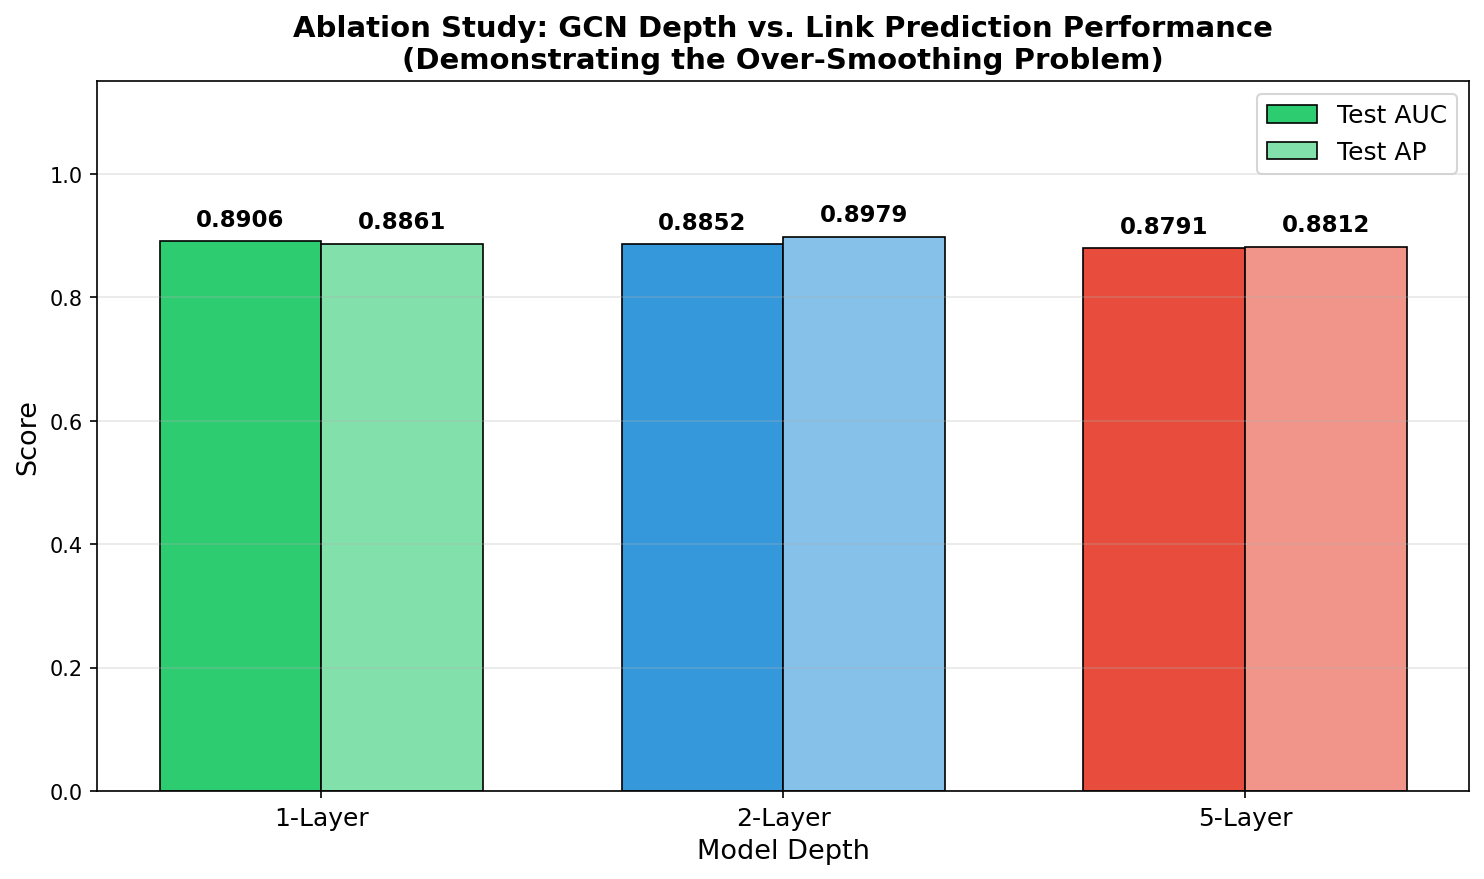
\includegraphics[width=\textwidth, height=0.42\textheight, keepaspectratio]{ablation_results.png}\\
{\tiny\textbf{GCN Depth}: 1L$\to$AUC=0.891;
2L$\to$0.885; 5L$\to$0.879 --- deeper = \alert{over-smoothing}}
\end{column}
\begin{column}{0.44\textwidth}
\begin{alertblock}{Over-Smoothing Explained}
Each GCN layer averages over the neighbourhood.
After 5 layers every node has absorbed its 5-hop neighbourhood --- embeddings converge to one vector.
\textbf{Prescription: Use 2-layer GCNs for sparse graphs.}
\end{alertblock}
\vspace{0.3em}
\begin{center}
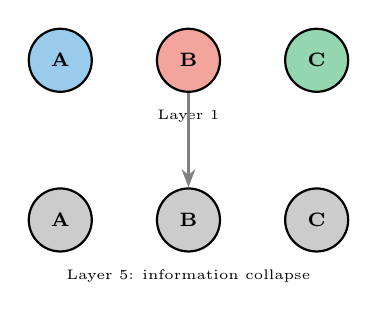
\begin{tikzpicture}[node distance=0.8cm]
\node[nd style, fill=cblue!50]   (a1) {A};
\node[nd style, fill=gapred!50,  right=of a1] (b1) {B};
\node[nd style, fill=fixgreen!50,right=of b1] (c1) {C};
\node[below=0.1cm of b1, font=\tiny]{Layer 1};
\node[nd style, fill=gray!40, below=1.2cm of a1] (a5) {A};
\node[nd style, fill=gray!40, right=of a5]        (b5) {B};
\node[nd style, fill=gray!40, right=of b5]        (c5) {C};
\node[below=0.1cm of b5, font=\tiny]{Layer 5: information collapse};
\draw[-{Stealth}, thick, gray] (b1) -- (b5);
\end{tikzpicture}
\end{center}
\end{column}
\end{columns}
\textbf{[O7 fully addressed]}
\end{frame}

% ============ F22: LEARNING CURVES ============
\begin{frame}
\frametitle{Results: Learning Curves}
\begin{center}
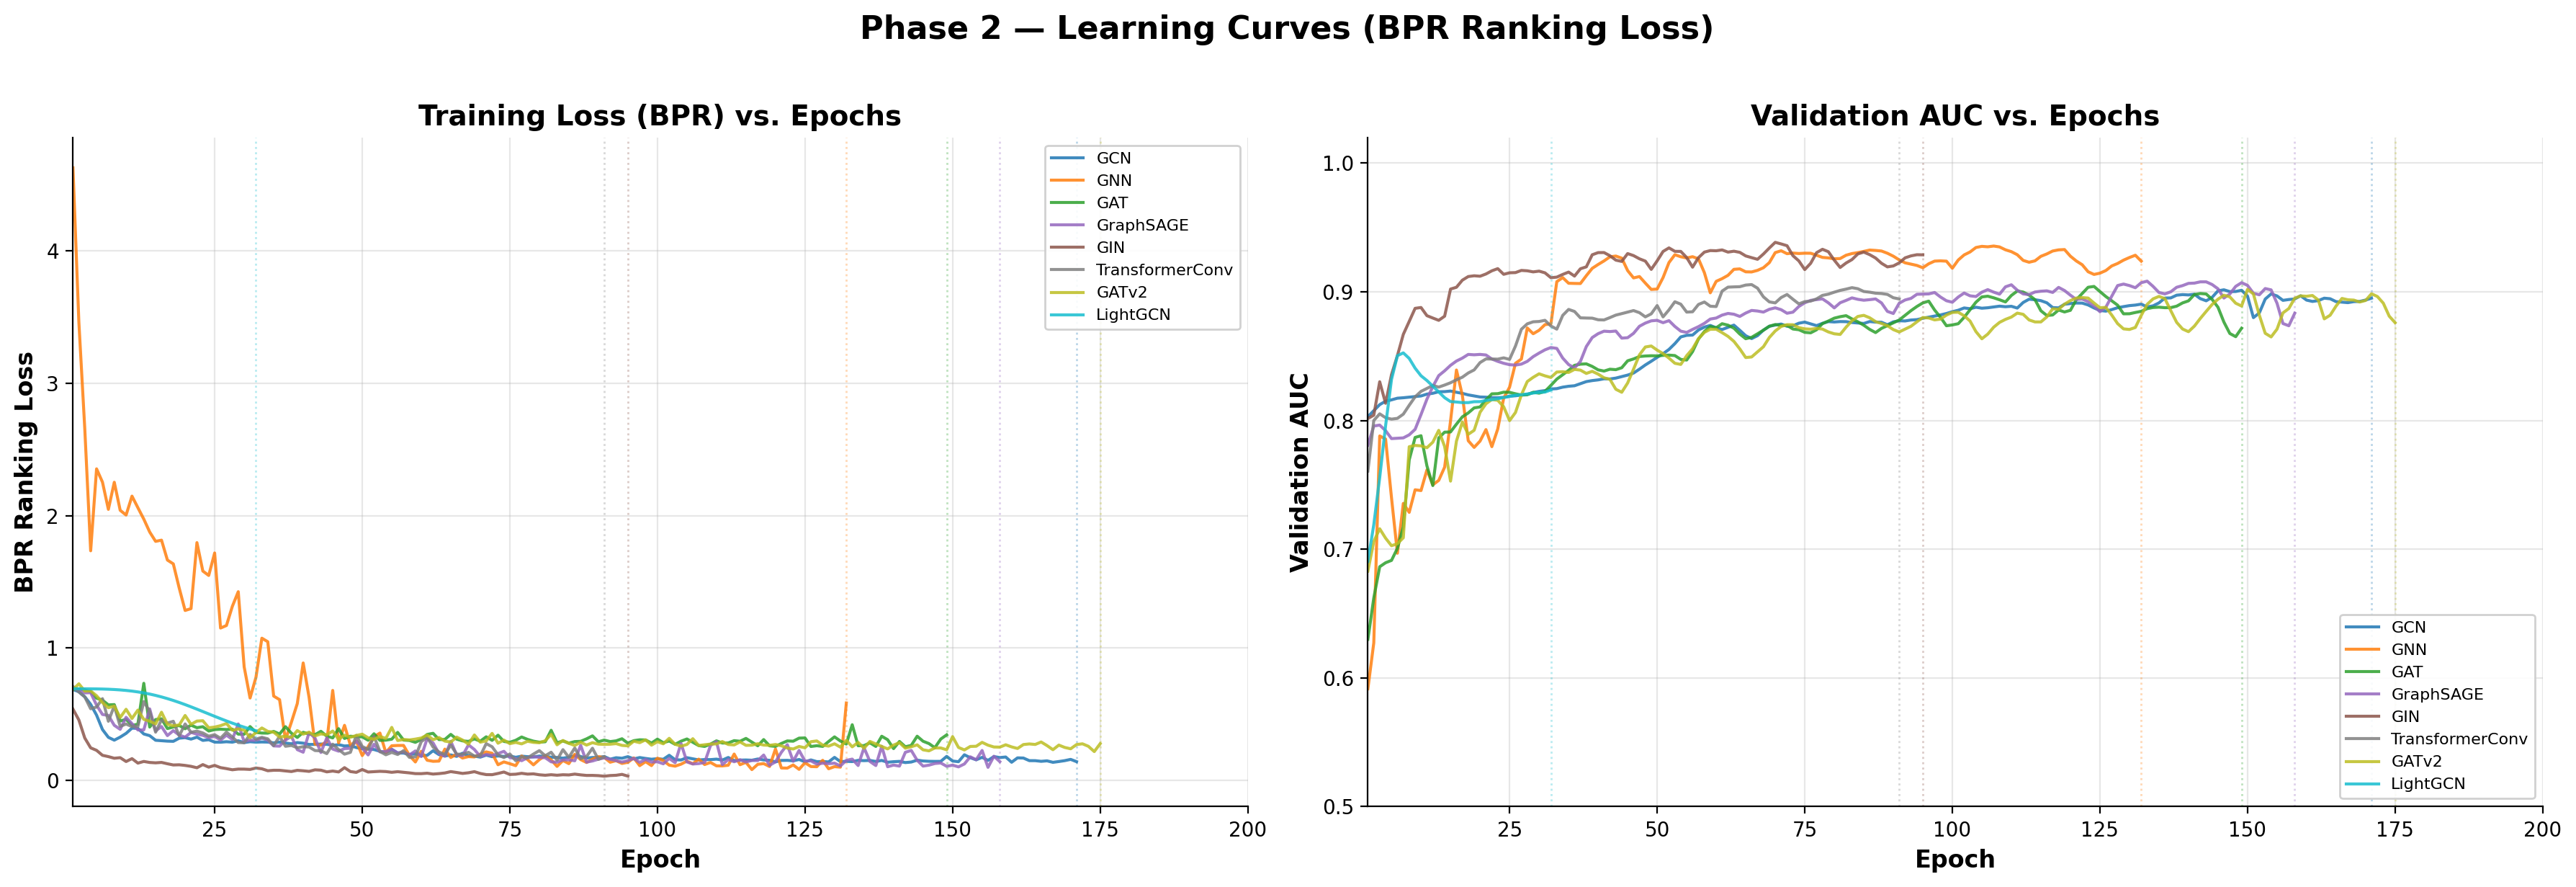
\includegraphics[width=\textwidth, height=0.6\textheight, keepaspectratio]{learning_curves_phase2.png}\\
{\scriptsize Phase 2 --- all 8 models stable, no overfitting.}
\end{center}
\begin{columns}[T]
\begin{column}{0.48\textwidth}
\begin{block}{Convergence}
\scriptsize All 8 models converge safely.
GNN largest initial BPR loss ($\sim$4.5), best Val AUC=0.933. LightGCN fastest (32 ep), GATv2 slowest (175 ep).
\end{block}
\end{column}
\begin{column}{0.48\textwidth}
\begin{block}{Regularisation}
\scriptsize Dropout=0.3 + patience=25 prevented overfitting. Val AUC plateaus smoothly after epoch 100. GIN early-stops at ep 95, saves 105 wasted epochs.
\end{block}
\end{column}
\end{columns}
\end{frame}

% ============ F23: DISCUSSION ============
\begin{frame}
\frametitle{Discussion: Which Architecture to Deploy?}
\begin{block}{Use Case 1 --- Maximise Ranking [O1]}
Winner: \textbf{GNN} nDCG=0.422, Recall=0.570, 8.3ms, 105K params.
Linear GraphConv + 2-layer MLP = right balance for sparse graphs.
\end{block}
\begin{block}{Use Case 2 --- Cold-Start / New Users [O1]}
Winner: \textbf{GIN}. Low-Deg Recall=0.771.
Injective MLP produces unique embeddings even for 1--2 neighbours.
\end{block}
\begin{block}{Use Case 3 --- Scale / Low Latency [O4]}
Winner: \textbf{LightGCN}.
5.3ms, 22K params. Only when latency strictly dominates accuracy (nDCG=0.221).
\end{block}
\begin{alertblock}{Avoid in Production:}
GATv2: 425K params, 29ms, nDCG=0.229 --- poor ROI.
GAT: collapses for users with fewer than 3 neighbours.
\end{alertblock}
\end{frame}

% ============ F24: DEPLOYMENT ============
\begin{frame}
\frametitle{Deployment: Real-Time REST API}
\begin{columns}[T]
\begin{column}{0.48\textwidth}
\begin{center}
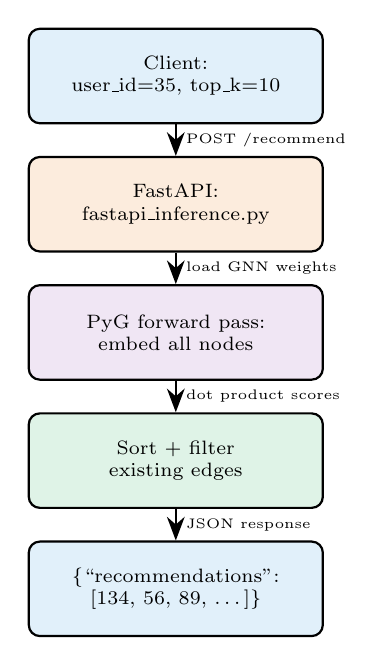
\begin{tikzpicture}[node distance=0.4cm]
\node[box style, fill=cblue!15, text width=3.5cm]   (c1) {Client:\\user\_id=35, top\_k=10};
\node[box style, fill=accent!15, text width=3.5cm, below=of c1]  (c2) {FastAPI:\\fastapi\_inference.py};
\node[box style, fill=cpurple!15, text width=3.5cm, below=of c2] (c3) {PyG forward pass:\\embed all nodes};
\node[box style, fill=fixgreen!15, text width=3.5cm, below=of c3] (c4) {Sort + filter\\existing edges};
\node[box style, fill=cblue!15, text width=3.5cm, below=of c4]   (c5) {\{``recommendations'':\\ {[134, 56, 89, \dots]}\}};
\draw[arr style] (c1)--(c2) node[midway, right, font=\tiny]{POST /recommend};
\draw[arr style] (c2)--(c3) node[midway, right, font=\tiny]{load GNN weights};
\draw[arr style] (c3)--(c4) node[midway, right, font=\tiny]{dot product scores};
\draw[arr style] (c4)--(c5) node[midway, right, font=\tiny]{JSON response};
\end{tikzpicture}
\end{center}
\end{column}
\begin{column}{0.48\textwidth}
\begin{block}{Specification}
\small
\textbf{Model:} GNN (winner by nDCG)\\
\textbf{Endpoint:} POST /recommend\\
\textbf{Input:} \{user\_id: int, top\_k: int\}\\
\textbf{Output:} ranked candidate node ID list\\
\textbf{Inference:} sub-100ms for 4,039-node graph\\[6pt]
Bridges ML research and production engineering.
\end{block}
\end{column}
\end{columns}
\end{frame}

% ============ F25: CONCLUSION ============
\begin{frame}
\frametitle{Conclusion}
\begin{alertblock}{1.\ BCE $\to$ BPR is Non-Negotiable}
Classification loss cannot optimise ranking.
nDCG/Recall tell the real story --- AUC alone is insufficient for recommendation evaluation.
\end{alertblock}
\begin{alertblock}{2.\ Feature Engineering Matters Without Profiles}
Adding Degree + PageRank improved nDCG from 0.419 to \textbf{0.430} (+2.6\%). Topology \emph{is} the feature.
\end{alertblock}
\begin{alertblock}{3.\ Architecture Verdict}
\begin{itemize}
  \item \textbf{Best accuracy + cold-start}: GNN / GIN
  \item \textbf{Best for scale}: LightGCN (5.3ms, 22K params)
  \item \textbf{Avoid}: GAT family for sparse graphs
\end{itemize}
\end{alertblock}
\end{frame}

% ============ F26: REFERENCES ============
\begin{frame}[allowframebreaks]
\frametitle{References}
\begin{thebibliography}{7}
\bibitem{kipf2017}
T.~Kipf and M.~Welling, ``Semi-Supervised Classification with Graph Convolutional Networks,'' \emph{ICLR}, 2017.
\bibitem{hamilton2017}
W.~Hamilton, Z.~Ying, and J.~Leskovec, ``Inductive Representation Learning on Large Graphs,'' \emph{NeurIPS}, 2017.
\bibitem{xu2019}
K.~Xu et al., ``How Powerful are Graph Neural Networks?'' \emph{ICLR}, 2019.
\bibitem{he2020}
X.~He et al., ``LightGCN: Simplifying and Powering GCN for Recommendation,'' \emph{SIGIR}, 2020.
\bibitem{brody2022}
S.~Brody, U.~Alon, and E.~Yahav, ``How Attentive are Graph Attention Networks?'' \emph{ICLR}, 2022.
\bibitem{rendle2009}
S.~Rendle et al., ``BPR: Bayesian Personalized Ranking from Implicit Feedback,'' \emph{UAI}, 2009.
\bibitem{maaten2008}
L.~van der Maaten and 
G.~Hinton, ``Visualizing Data using t-SNE,'' \emph{JMLR}, 2008.
\end{thebibliography}
\end{frame}

% ============ F27: THANK YOU ============
\begin{frame}[standout]
\Huge Thank You\\[12pt]
\Large Open to Questions\\[16pt]
\normalsize Group 47\enspace$\vert$\enspace NIT Patna\\[4pt]
Guide: Dr.\ Mukesh Kumar
\end{frame}

\end{document}